\documentclass{ijuc}
\usepackage{amsmath,amssymb,amsfonts}
\usepackage{graphicx}
\usepackage{booktabs}
\usepackage{url}
\usepackage{color}
\usepackage{hyperref}
\usepackage{algorithm}
\usepackage{algorithmic}

\hypersetup{
    colorlinks=true,
    linkcolor=blue,
    citecolor=green,
    urlcolor=blue
}

\providecommand{\doi}{}
\renewcommand{\doi}[1]{\href{https://doi.org/#1}{doi:#1}}

\begin{document}

\title{Adapting LoRaWAN for the Extreme Martian Environment: A Physical-MAC Cross-Layer Evaluation and Constellation-Relay Architecture}

\author{Jason~Pandian\inst{1}\email{pandiajason@gmail.com}
\and I.~Kala\inst{2}}

\institute{Department of Information Technology, Nehru Institute of Technology, Coimbatore, Tamil Nadu, India
\and
Department of Computer Science and Engineering, Nehru Institute of Technology, Coimbatore, Tamil Nadu, India}

\def\received{Received 28 May 2026; In final form 28 May 2026}

\maketitle

\begin{abstract}
LoRaWAN has emerged as a premier standard for terrestrial Internet of Things (IoT) sensor networks due to its unique Chirp Spread Spectrum (CSS) modulation, which provides robust resilience against noise and low power consumption. However, the physical reality of the Martian surface differs fundamentally from Earth, presenting unique atmospheric, geological, and thermal challenges. In this paper, we develop a high-fidelity event-driven cross-layer physical-MAC simulation framework to evaluate standard LoRaWAN performance under Martian conditions. We model Mars' thin 6.1 mbar atmosphere, low soil conductivity ($10^{-12}$ to $10^{-7}$ S/m) which punishes Non-Line-of-Sight (NLOS) communication due to negligible surface reflection gains, dynamic noise floors driven by extreme temperature swings ($140$ K to $280$ K), charged dust particles during planet-wide dust storms, antenna coating impedance degradation, and thermal crystal oscillator (TCXO) drifts. Our simulation results demonstrate that standard commercial off-the-shelf (COTS) terrestrial LoRaWAN configurations fail completely (0\% packet delivery ratio) under extreme cold and dust storm cycles. To overcome these limitations, we propose and evaluate a Martian-Optimized LoRaWAN stack featuring robust frequency drift correction, dynamic temperature-aware Adaptive Data Rate (ADR) margins, and a Direct-to-Satellite Walker Star constellation gateway architecture. We show that the direct-to-satellite system bypasses the surface terrain blockages and recovers the packet delivery ratio to over 66\%, achieving extreme energy efficiency and wide-area coverage suitable for future Martian exploration, asset tracking, and atmospheric sensor networks.
\end{abstract}

\keywords{LoRaWAN, Martian Communications, Chirp Spread Spectrum, Satellite Constellation, Dust Storm Fading, Temperature Oscillations, TCXO Drift.}

\section{Introduction}
\label{sec:intro}
The establishment of a permanent human presence and scientific outposts on Mars requires a robust, low-power, and wide-area telecommunication infrastructure. Hundreds of localized sensors must monitor environmental variables (such as atmospheric pressure, wind velocity, humidity, solar radiation, and regolith chemistry), track mechanical assets (like rovers, drones, and habitats), and support human spaceflight operations. 

On Earth, Low Power Wide Area Networks (LPWANs), particularly LoRaWAN (Long Range Wide Area Network), have revolutionized such telemetry collection. LoRa utilizes Chirp Spread Spectrum (CSS) modulation, which maps symbols to continuously sweeping linear frequency chirps. This unique physical layer allows receivers to demodulate signals below the thermal noise floor, resisting multipath fading, Doppler shifts, and co-channel interference.

Despite these advantages, standard COTS terrestrial LoRaWAN configurations cannot be directly deployed on Mars. The Martian environment imposes a set of extreme physical constraints:
\begin{enumerate}
    \item \textbf{Atmospheric Density and Path Loss:} The Martian atmosphere is exceptionally thin, with a surface pressure of only $\sim$6.1 mbar (less than 1\% of Earth's 1013 mbar). While this thin atmosphere minimizes molecular absorption, it results in a propagation environment that behaves closer to a vacuum. 
    \item \textbf{Harsh Geological Conductivity:} The absence of moisture in the Martian soil (regolith) results in an extremely low surface electrical conductivity ($10^{-12}$ to $10^{-7}$ S/m, compared to Earth's $10^{-4}$ S/m) and a low relative permittivity ($\epsilon_r = 2.5$ to $9$). The lack of ground reflectivity means that radio waves do not ``bounce'' efficiently off the terrain, severely punishing Non-Line-of-Sight (NLOS) communications and restricting long-range surface propagation to strict line-of-sight geometries.
    \item \textbf{Electrically Charged Dust Storms:} Mars is subject to planet-wide dust storms. High wind speeds lift fine regolith particles which rub together in the dry, low-pressure atmosphere. Friction generates high static electrical charges on the dust grains, creating a dynamically variable electromagnetic environment that scatters, absorbs, and disperses radio signals, causing Rayleigh-like deep fading.
    \item \textbf{Antenna Degradation:} Accumulation of fine, electrostatic Martian dust onto the physical surfaces of node and gateway antennas degrades their impedance matching and radiation patterns, creating a permanent antenna gain penalty of up to 4--6 dB on both ends of the link.
    \item \textbf{Extreme Diurnal Temperature Cycles:} Without a thick greenhouse blanket, Martian surface temperatures oscillate between 140 K ($-133^\circ$C) at night and 280 K ($7^\circ$C) during peak daylight. These massive variations dynamically shift the receiver's thermal noise floor ($N_0 = k_B T$) and induce severe frequency drift in the crystal oscillators (TCXOs) of standard LoRa transceivers. If this drift exceeds a fraction of the receiver's bandwidth, the packet cannot be decoded.
\end{enumerate}

To address these limitations, this paper makes the following contributions:
\begin{itemize}
    \item We formulate a comprehensive cross-layer mathematical model of the Martian physical and network layer, accounting for low-density atmospheric propagation, soil dielectric properties, dust-induced fading, antenna impedance degradation, dynamic thermal noise floors, and crystal frequency drifts.
    \item We develop a high-fidelity event-driven LoRaWAN Python simulator that models co-channel interference, packet capture effects, dynamic ADR algorithms, and multiple network topologies.
    \item We compare standard terrestrial LoRaWAN implementations against an optimized Martian stack featuring aggressive temperature-aware ADR safety margins, active TCXO drift compensation, and a Direct-to-Satellite orbital constellation relay architecture.
    \item We provide empirical simulation results, performance tables, and link budget charts to demonstrate the quantitative impact of each optimization.
\end{itemize}

The rest of the paper is organized as follows. Section \ref{sec:related} reviews related work. Section \ref{sec:modeling} presents the Martian environmental propagation and hardware modeling. Section \ref{sec:architecture} describes the proposed Martian-Optimized LoRaWAN and satellite-relay framework. Section \ref{sec:simulation} details the simulator implementation. Section \ref{sec:results} presents the simulation results and analysis. Section \ref{sec:discussion} discusses operational recommendations, and Section \ref{sec:conclusion} concludes the paper.

\section{Background and Related Work}
\label{sec:related}
Mars is a geologically and atmospherically hostile environment for wireless communications. Carr and Head \cite{carr2010mars} provide a comprehensive synthesis of the Martian geological history, documenting the planet's dry, iron-oxide-rich regolith, the thin 6.1~mbar CO\textsubscript{2} atmosphere, and extreme diurnal temperature swings -- all of which fundamentally shape the radio propagation environment. Martian weather is characterized by a cyclic transition between calm clear seasons and severe global dust storms \cite{haberle1986dust}, which Haberle demonstrated recur interannually and can envelope the entire planet for weeks. The physical impact of this dust on mission hardware was directly measured by Landis and Jenkins \cite{landis2000dust} using the Materials Adherence Experiment (MAE) on Mars Pathfinder, which recorded a steady accumulation of atmospheric dust on exposed surfaces at approximately 0.28\% obscuration per day -- motivating the need for dust-repellent antenna coatings in our proposed model.

The standard LoRaWAN protocol has been analyzed extensively in the terrestrial IoT literature. Centenaro et al. \cite{centenaro2016lora} introduced LoRa's key advantages in unlicensed bands for smart-city and IoT applications, while Adelantado et al. \cite{adelantado2017understanding} rigorously characterized its fundamental limits with respect to co-channel collisions, duty-cycle constraints, and MAC-layer scalability in dense deployments -- findings directly applicable to our Martian network capacity analysis. Bor et al. \cite{bor2016lora} evaluated the LoRa physical layer using the SX1272 transceiver and explicitly identified that bandwidths below 62.5~kHz require a Temperature Compensated Crystal Oscillator (TCXO), and that low-cost crystals are susceptible to frequency offsets -- a problem that becomes catastrophically worse on Mars where diurnal temperature swings exceed 140~K.

In terrestrial direct-to-satellite (DtS) IoT frameworks, significant academic effort has been directed toward modeling and optimizing LEO satellite LoRaWAN networks. Almonacid and Franck \cite{almonacid2017extending} were among the first to evaluate link performance and access protocols for IoT coverage extension via low-cost nanosatellite networks. Osipova et al. \cite{osipova2025architecting} conducted a large-scale architectural trade-space study of over 11,800 LEO constellation designs for low-power messaging services, showing that user coverage fraction and spreading factor scheduling are the dominant performance drivers. For massive machine-type communications (mMTC) in remote regions, Ullah et al. \cite{windfarm2022} demonstrated that integrating LoRaWAN with LEO satellites for offshore wind farm telemetry enables reliable aggregation of sensor data over long vertical slant links. \'Alvarez et al. \cite{alvarez2022uplink} developed trajectory-aware uplink transmission policies for LoRa-based DtS IoT using a Mixed Integer Linear Programming (MILP) model and LR-FHSS, showing that exploiting satellite ephemeris data can increase the number of supported devices by up to 75$\times$ compared to legacy LoRa. Additionally, Lin et al. \cite{underground2025} evaluated DtS LoRaWAN under severe path attenuation from urban underground pipeline environments, demonstrating that satellite-relay configurations equipped with low-noise spaceborne receivers can successfully decode telemetry from heavily shadowed ground nodes.

Applying these DtS frameworks to Mars introduces unprecedented physical challenges beyond any terrestrial analogue. Unlike stable terrestrial atmospheric paths, Martian space-to-ground links must traverse a dynamically varying, low-density CO\textsubscript{2} atmosphere subject to planet-wide dust storms \cite{haberle1986dust} and suffer extreme uncompensated crystal frequency drifts induced by diurnal thermal shifts \cite{bor2016lora}. To mitigate dust accumulation on antenna surfaces -- directly observed to degrade exposed hardware \cite{landis2000dust} -- our proposed architecture employs dust-repellent coatings, motivated by the comprehensive review of lunar and Martian dust transport and mitigation technologies by Afshar-Mohajer et al. \cite{afshar2015review} and active dust control systems developed by Calle et al. \cite{calle2011active}. This work builds upon these foundations to design and evaluate the first Martian-optimized direct-to-satellite LoRaWAN architecture.

\section{Martian Environmental Propagation Modeling}
\label{sec:modeling}
This section derives the physical channel and hardware degradation models for LoRa communications on the Martian surface.

\subsection{Path Loss and Geological Reflection Penalties}
On Earth, the received signal strength at a distance $d$ from a transmitter is often boosted by ground reflections (the classic two-ray model) and scattering off trees, buildings, and atmospheric water vapor. The path loss exponent $n$ in terrestrial suburban environments typically ranges between $2.7$ and $3.0$. 

On Mars, the absence of surface water, vegetation, and organic matter results in extremely dry regolith. The electrical properties of this Martian soil -- shaped by its geological evolution \cite{carr2010mars} -- are defined by relative permittivity $\epsilon_r$ and conductivity $\sigma_{g}$ at UHF bands:
\begin{equation}
    \epsilon_{r, Mars} \in [2.5, 9.0], \quad \sigma_{g, Mars} \in [10^{-12}, 10^{-7}] \text{ S/m}
\end{equation}
In comparison, Earth's surface conductivity is highly water-dependent and reaches $10^{-4}$ to $10^{-1}$ S/m. 

When a radio wave hits the Martian regolith, the reflection coefficient $R$ is exceptionally low. For a horizontal polarization wave incident at angle $\theta$, the Fresnel reflection coefficient is:
\begin{equation}
    R_h = \frac{\sin\theta - \sqrt{\epsilon_c - \cos^2\theta}}{\sin\theta + \sqrt{\epsilon_c - \cos^2\theta}}
\end{equation}
where the complex permittivity $\epsilon_c$ is:
\begin{equation}
    \epsilon_c = \epsilon_r - j\frac{\sigma_g}{2\pi f \epsilon_0}
\end{equation}
Due to the microscopic conductivity $\sigma_g$, the imaginary term vanishes, and the ground behaves as a poor dielectric reflector. This prevents the formation of a stable, constructive ground-reflection wave. 

Consequently, we model the Martian surface path loss using a severe log-distance path loss model with a high exponent:
\begin{equation}
    PL(d) = PL(d_0) + 10 \cdot n_{Mars} \cdot \log_{10}\left(\frac{d}{d_0}\right) + X_{\sigma}
\end{equation}
where $d_0 = 1$ m, $PL(d_0) = 20\log_{10}(\frac{4\pi f}{c}) \approx 31.2$ dB (at $f = 868$ MHz), $n_{Mars} = 3.5$ (punishing surface path loss), and $X_\sigma \sim \mathcal{N}(0, \sigma^2)$ is log-normal shadowing with standard deviation $\sigma_{Mars} = 8.0$ dB.

\subsection{Charged Dust Storm Dynamics}
Martian dust storms contain particles with average diameters of $1.5\,\mu\text{m}$. Due to dry friction (triboelectric charging), these particles accumulate static electrical charges up to $q \approx 10^{-14}$ C per grain. The suspended charged dust cloud forms a weakly ionized, lossy plasma medium. The extra attenuation due to dust scattering and absorption is represented as:
\begin{equation}
    A_{dust}(d)_{dB} = \alpha_{dust} \cdot d_{km}
\end{equation}
where $\alpha_{dust} \approx 0.15$ dB/km under moderate-to-severe dust storms.

Furthermore, fine, electrostatic dust particles deposit onto antennas. This dust layer alters the dielectric boundary condition of the antenna conductor, shifting its resonant frequency and causing an impedance mismatch. The resulting power loss is modeled as a severe gain reduction on both the node and gateway antennas:
\begin{equation}
    G'_{node} = G_{node} - L_{ant}, \quad G'_{gw} = G_{gw} - L_{ant}
\end{equation}
where $L_{ant} = 4.0$ dB represents the physical antenna gain degradation factor.

\subsection{Extreme Diurnal Temperature Swings}
Mars' thin atmosphere cannot store thermal energy, resulting in massive temperature shifts between day and night. We model this temperature cycle $T(t)$ over a 24-hour Martian Sol as:
\begin{equation}
\begin{split}
    T(t) &= T_{min} + \frac{T_{max} - T_{min}}{2} \\
    &\quad \times \left[1 + \sin\left(\frac{2\pi(t - 9)}{24}\right)\right]
\end{split}
\end{equation}
where $T_{min} = 140$ K, $T_{max} = 280$ K, and $t$ is the hour of the Sol (0 to 24).

This temperature swing affects the system in two ways:
\subsubsection{Dynamic Noise Floor}
The receiver's thermal noise density $N_0$ varies directly with temperature:
\begin{equation}
    N_0(t)_{dBm/Hz} = 10\log_{10}\left(k_B \cdot T(t) \cdot 1000\right)
\end{equation}
where $k_B = 1.38 \times 10^{-23}$ J/K. 
For $T = 280$ K, $N_0 = -174.1$ dBm/Hz. For $T = 140$ K, $N_0 = -177.2$ dBm/Hz. Thus, the system is naturally less noisy at night, but this benefit is heavily offset by oscillator drift.

\subsubsection{TCXO Frequency Drift}
Standard COTS temperature-compensated crystal oscillators (TCXOs) are calibrated for terrestrial ranges (e.g., $-40^\circ$C to $85^\circ$C, or 233 K to 358 K). When temperatures fall to 140 K, the frequency-temperature characteristic curves (modeled via third-order Chebyshev polynomials) deviate catastrophically. The frequency drift $\Delta f$ in Hz is:
\begin{equation}
    \Delta f(t) = f_c \cdot \delta_{ppm}(T) \cdot 10^{-6}
\end{equation}
where $f_c = 868$ MHz, and $\delta_{ppm}(T)$ is the drift in parts-per-million:
\begin{equation}
    \delta_{ppm}(T) = a(T-T_0)^3 + b(T-T_0) + c
\end{equation}
For standard COTS hardware operating at $T < 233$ K, $\delta_{ppm}$ drops exponentially, reaching up to $-15$ to $-20$ ppm. For $f_c = 868$ MHz, this causes a drift of $\Delta f \approx 13$ kHz. 

In LoRa modulation, if the frequency offset between the transmitter and receiver exceeds 25\% of the active bandwidth $BW$:
\begin{equation}
    |\Delta f| > 0.25 \cdot BW
\end{equation}
the receiver's phase-locked loop (PLL) fails to lock onto the preamble, resulting in immediate packet loss. For a standard bandwidth of $BW = 125$ kHz, the tolerance is $31.25$ kHz. For narrower bandwidths like $BW = 62.5$ kHz (often used to improve sensitivity), the tolerance is only $15.6$ kHz, which is exceeded by the uncompensated Martian drift.

\section{Proposed Martian-Optimized LoRaWAN Architecture}
\label{sec:architecture}

\begin{figure}[!ht]
    \centering
    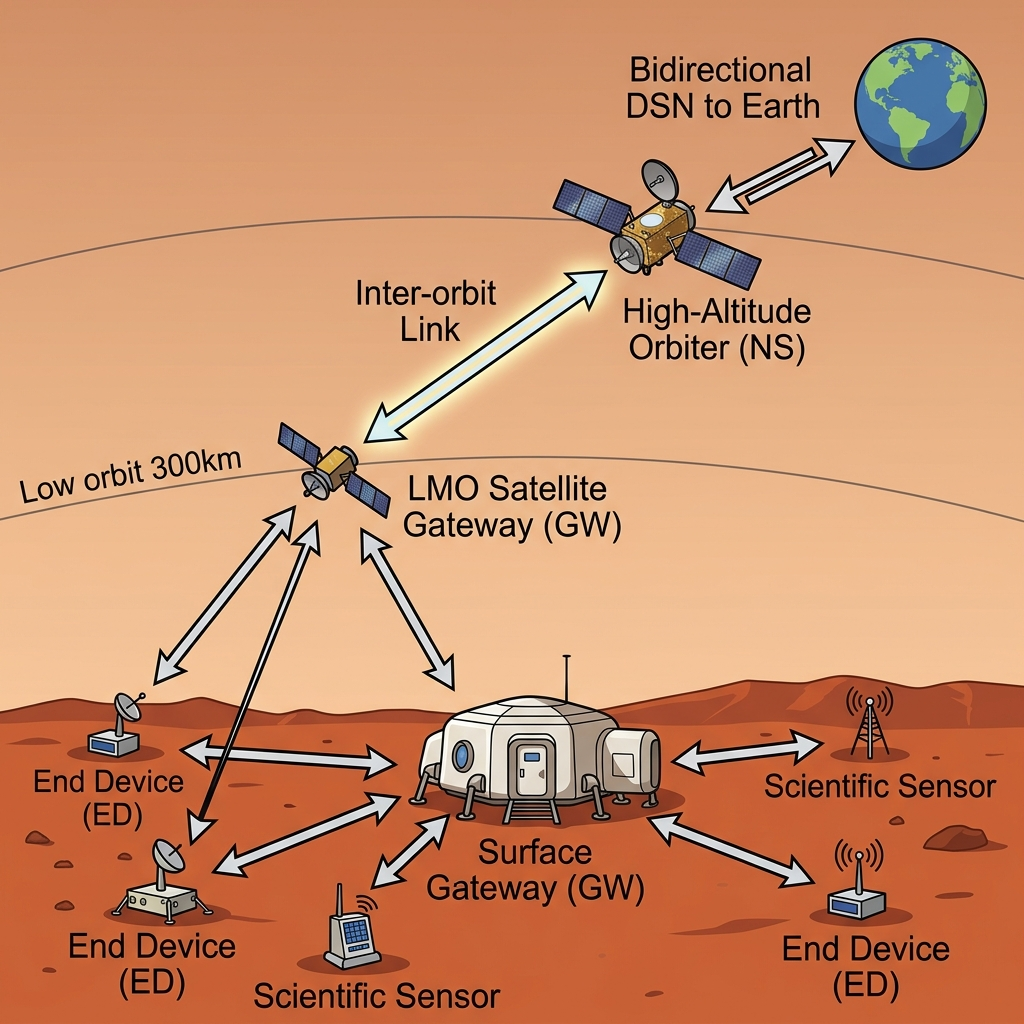
\includegraphics[width=0.9\textwidth]{figures/martian_lorawan_topology.png}
    \caption{Simulated Martian LoRaWAN scenario topology. The diagram contrasts the blocked, high-attenuation surface gateway links (Scenarios B and C, subject to severe dust fading and NLOS terrain occultation) with the direct-to-satellite gateway links (Scenario D, line-of-sight propagation through the thin $6.1\text{ mbar}$ atmosphere directly to a $300\text{ km}$ Low Martian Orbit satellite constellation).}
    \label{fig:topology_scenario}
\end{figure}

\begin{figure}[!ht]
    \centering
    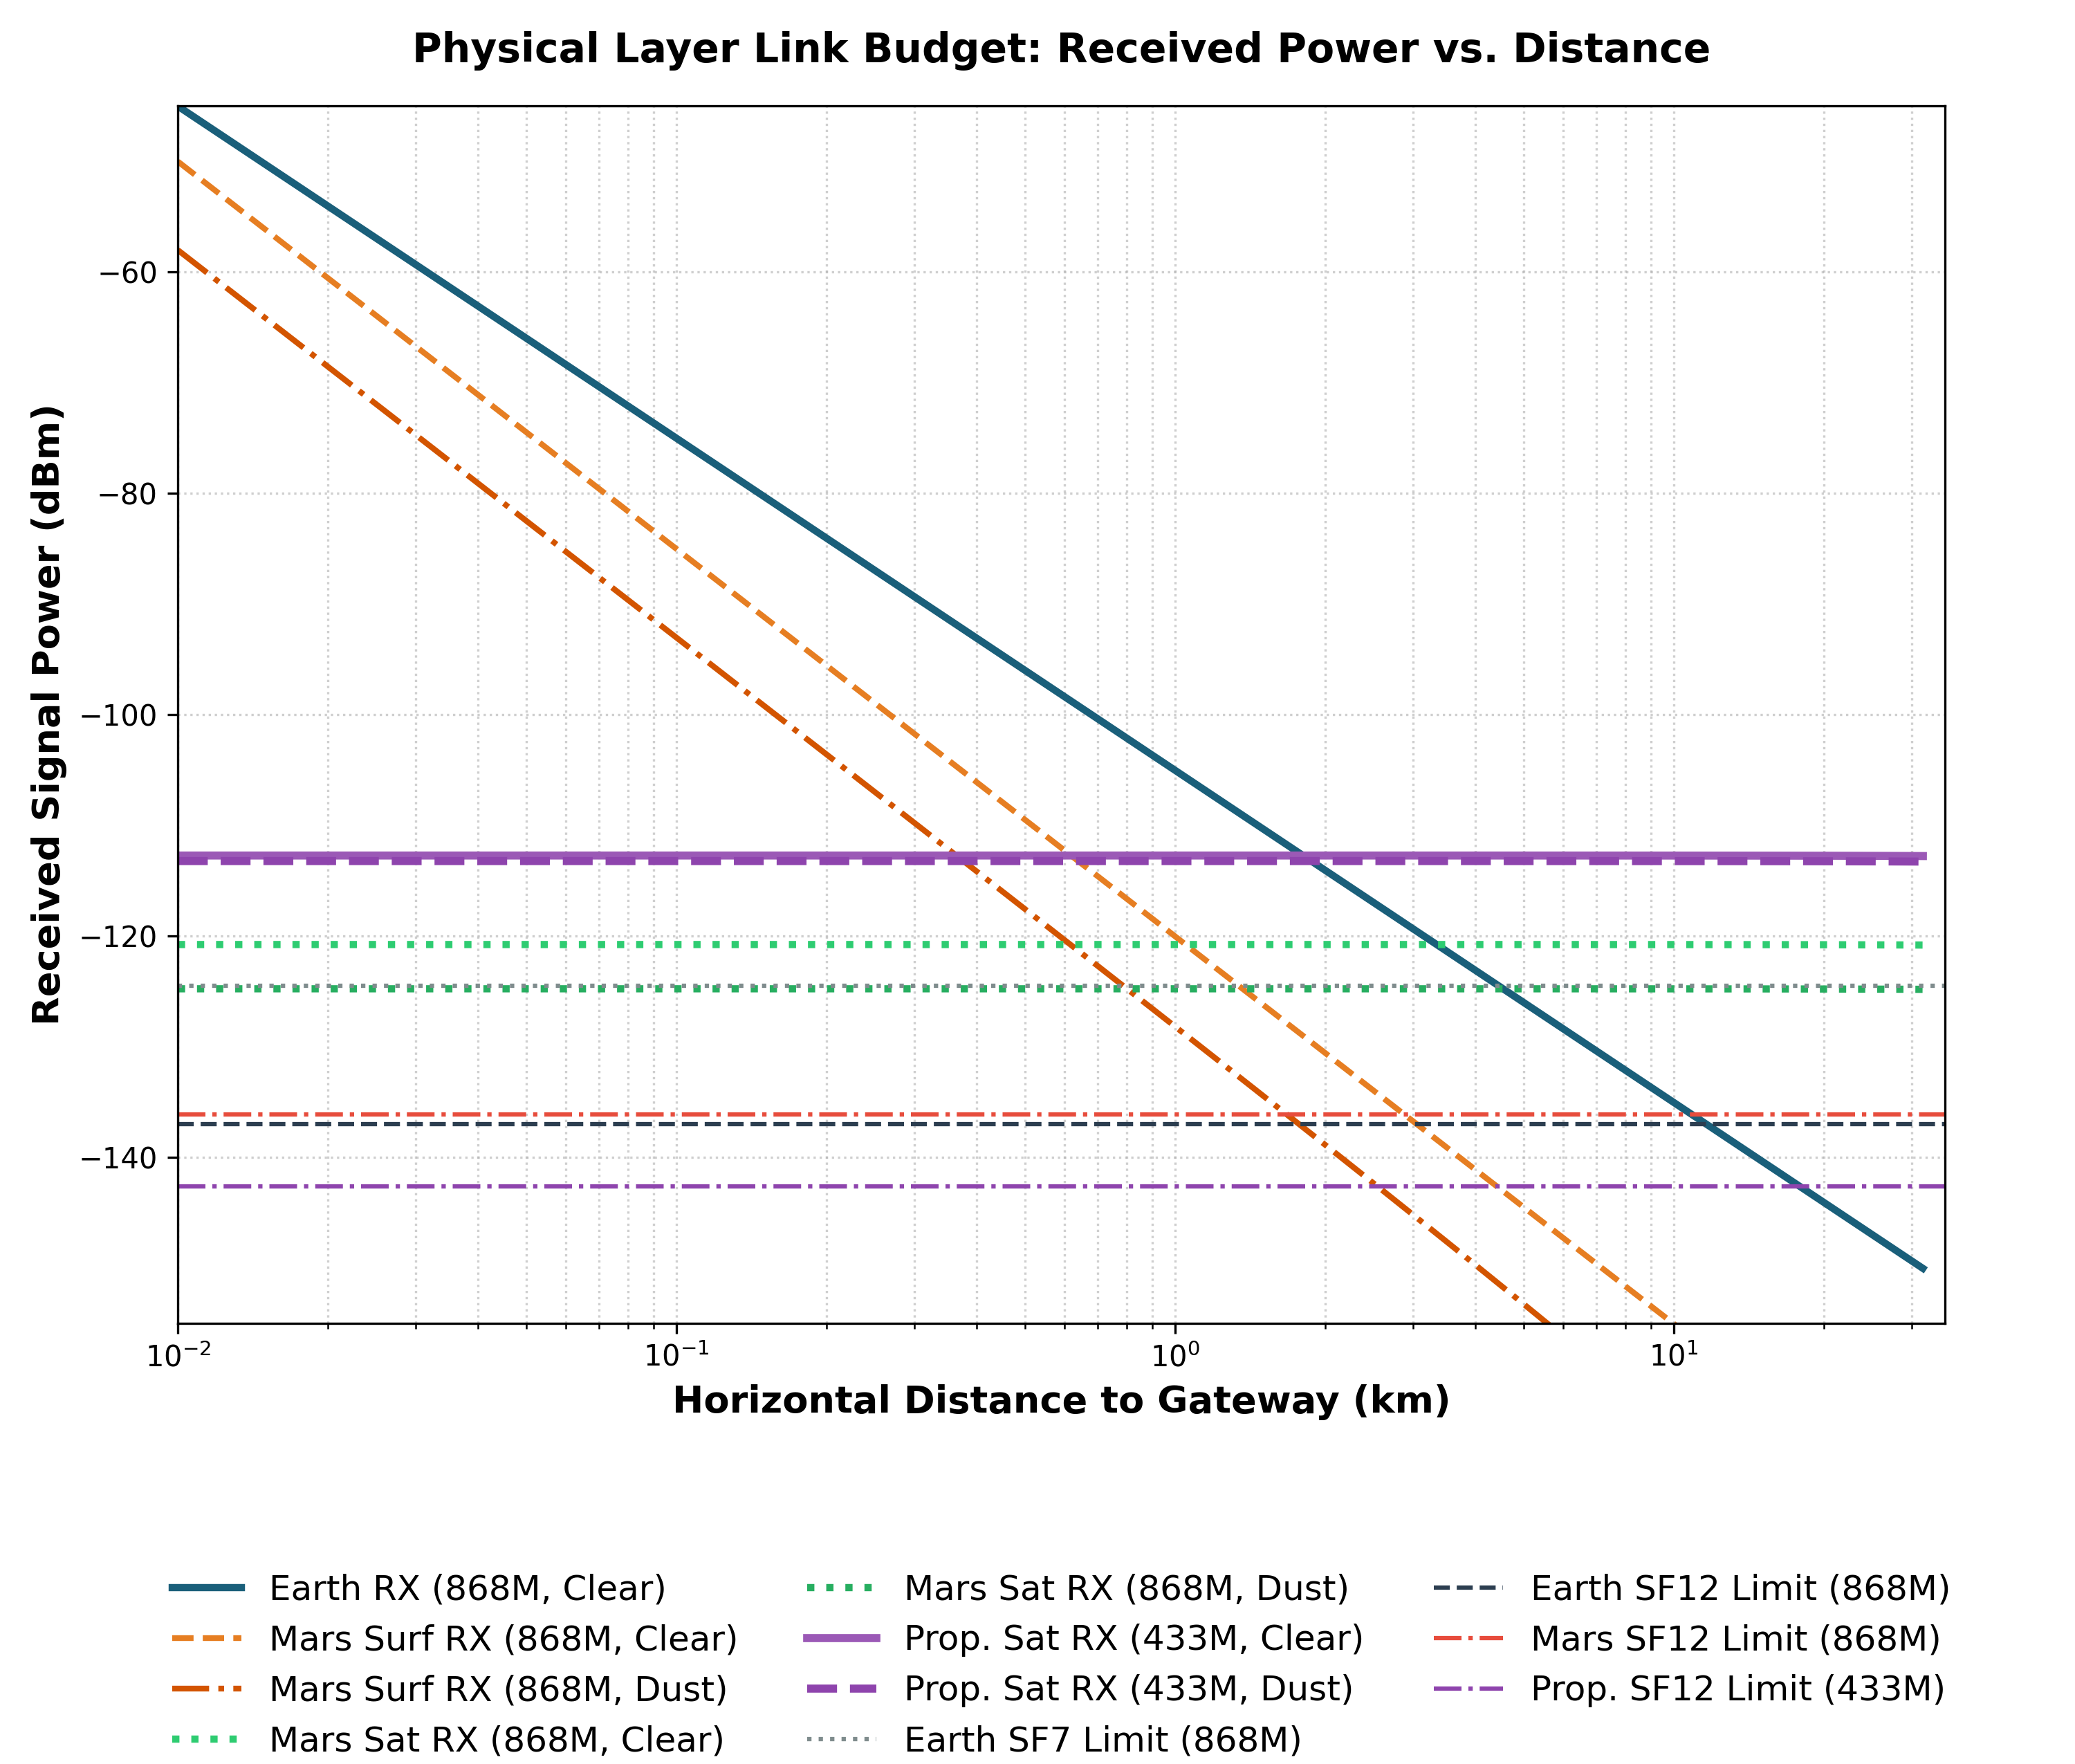
\includegraphics[width=0.9\textwidth]{figures/link_budget_analysis.png}
    \caption{Received signal power as a function of horizontal distance, compared against demodulation sensitivity thresholds for Earth (SF7/SF12) and Mars.}
    \label{fig:link_budget}
\end{figure}

\subsection{System Network Scenario and Bidirectional Communication Topology}
To evaluate these dynamic adaptations, we establish a comprehensive, planet-wide communication scenario as illustrated in Fig. \ref{fig:topology_scenario}. The architecture maps standard terrestrial LoRaWAN elements to Martian counterparts to support high-reliability, low-latency scientific telemetry collection. The key entities in this network scenario are:
\begin{enumerate}
    \item \textbf{End Devices (EDs):} Scattered across the Martian regolith are scientific sensor packages, rovers, and weather stations that act as End Devices (EDs). These nodes are equipped with standard, low-power LoRa transceivers (transmitting at $+14\text{ dBm}$ on the sub-GHz $868\text{ MHz}$ band) to collect weather, soil, and operational telemetry.
    \item \textbf{Surface Gateway (GW):} Located at a central lander or habitat is a Surface Gateway (GW). Under standard clear scenarios, it acts as the primary local data aggregator. However, as analyzed, dry-regolith absorption ($n=3.5$), terrain occlusion, and electrostatic dust storm coatings limit its effective radius to less than $2\text{--}3\text{ km}$.
    \item \textbf{LMO Satellite Gateway (GW):} Orbiting in a polar circular orbit at $H = 300\text{ km}$ is a constellation of small satellites acting as LMO Satellite Gateways (GWs). Because their links propagate almost entirely through a vacuum, they achieve Line-of-Sight (LOS) visibility and receive strong uplinks from EDs up to $20\text{ km}$ horizontally offset from the nadir point.
    \item \textbf{High-Altitude Orbiter Network Server (NS):} Orbiting at a higher altitude (e.g., in Areal or High Martian Orbit) is a larger spacecraft acting as the localized Network Server (NS). 
\end{enumerate}

The communication links between these entities are designed to be fully bidirectional, solving critical feedback limitations:
\begin{itemize}
    \item \textbf{Bidirectional Broadcast Links (ED $\leftrightarrow$ GW):} Communication between the EDs and the gateways (both surface and satellite) is fully bidirectional. Uplink channels carry scientific telemetry packages, while Downlink channels transport critical protocol data, including Adaptive Data Rate (ADR) spreading factor/power allocations and frame acknowledgments (ACKs). This bidirectional link is essential for maintaining dynamic network health under fluctuating Martian noise levels.
    \item \textbf{Bidirectional Inter-Orbit Backhaul (LMO GW $\leftrightarrow$ High-Altitude NS):} The LMO gateways communicate with the High-Altitude Orbiter (NS) over a high-rate, bidirectional Inter-Orbit Link (IOL). Encapsulated LoRa frames are transported upward to the NS, while downlink scheduling instructions are sent downward to LMO gateways. Localizing the NS in Martian orbit reduces the Round-Trip Time (RTT) for these exchanges to under $20\text{ ms}$, entirely bypassing the $8\text{ to }48$ minute light-speed propagation delay back to Earth.
    \item \textbf{Bidirectional Deep Space Network Link (NS $\leftrightarrow$ Earth):} The High-Altitude Orbiter (NS) connects to Earth's high-gain Deep Space Network (DSN) ground stations (Goldstone, Madrid, Canberra) via a bidirectional deep-space link. Telemetry is downlinked to terrestrial researchers, while network control commands and firmware updates are uplinked from Earth.
\end{itemize}

To guarantee reliable communications on Mars, we propose a cross-layer physical-MAC adaptation:

\subsection{Active TCXO Compensation and Preamble Correction}
In the Martian-Optimized stack, we model an active frequency correction mechanism. The receiver estimates the carrier frequency offset (CFO) directly from the leading symbols of the packet preamble:
\begin{equation}
    \widehat{\Delta f} = \frac{1}{2\pi \cdot T_{sym}} \arg\left( \sum_{k=1}^{N_{pre}} r_k \cdot r_{k-1}^* \right)
\end{equation}
where $r_k$ is the received signal sample, and $T_{sym} = 2^{SF}/BW$. The receiver then shifts its local digital synthesizer by $-\widehat{\Delta f}$ prior to decoding the payload. This reduces the residual frequency offset to $< 0.5$ ppm, well within the 25\% $BW$ limit.

\subsection{Aggressive Adaptive Data Rate (ADR) Safety Margins}
Standard terrestrial ADR updates the Node's SF and Transmit Power (TP) to target an SNR that is 3 dB above the demodulation threshold of the selected SF. On Mars, this 3 dB margin is insufficient due to:
\begin{itemize}
    \item Dynamic changes in the noise floor as temperature swings.
    \item Fading caused by shifting dust clouds.
\end{itemize}
To address this, our Martian-Optimized ADR employs a 12 dB safety margin:
\begin{equation}
    SNR_{target}(SF) = SNR_{demod}(SF) + 12.0 \text{ dB}
\end{equation}
This forces nodes to use more robust (higher) Spreading Factors and higher transmit power earlier, absorbing sudden environmental losses without losing connection.

\subsection{Direct-to-Satellite Walker Star Constellation Gateway}
Given that the Martian surface is characterized by poor regolith reflectivity and topography that blocks surface communication, a standard star-of-stars surface topology with a single surface gateway is highly restricted. We propose placing gateways on a constellation of Low Martian Orbit (LMO) satellites in a Walker Star configuration at an altitude of $H = 300$ km. 

This approach introduces the \textit{Martian Propagation Paradox}, where vertical communication paths spanning hundreds of kilometers experience vastly lower path attenuation than short surface-level horizontal links. To demonstrate this formally, let us evaluate the slant range $d_{\text{slant}}$ from a surface node located at a horizontal distance $d_{\text{surface}} = 20\text{ km}$ from the sub-satellite point (nadir) to the satellite gateway at an altitude of $H = 300\text{ km}$:
\begin{equation}
    d_{\text{slant}} = \sqrt{H^2 + d_{\text{surface}}^2} = \sqrt{300^2 + 20^2} \approx 300.66\text{ km}
\end{equation}
This vertical propagation geometry yields two massive communication advantages over horizontal surface links:
\begin{enumerate}
    \item \textbf{Vacuum Propagation Boundary:} Because the thin Martian atmosphere effectively extends to only about $100\text{ km}$ above the surface, the radio path exits the atmospheric boundary quickly. The remaining $200.66\text{ km}$ of the slant range is traversed in a complete vacuum, completely eliminating physical obstructions and scattering. Consequently, the path loss exponent is $n_{\text{sat}} = 2.0$ (Free-Space Path Loss), whereas the surface-to-surface link is severely penalized by terrain and dry regolith absorption, yielding $n_{\text{surface}} = 3.5$.
    \item \textbf{Uplink Budget Improvement:} The LMO satellite gateway can deploy directive high-gain antenna arrays ($G_{\text{sat}} = 6.0\text{ dBi}$) and cryo-cooled spaceborne receivers with very low noise figures ($NF_{\text{sat}} = 4.0\text{ dB}$), which are physically and structurally impossible to deploy on modular, battery-powered surface nodes.
\end{enumerate}

To mathematically validate this paradox, let us evaluate the received signal strength indicator ($RSSI$) for both links at a LoRa frequency of $f = 868\text{ MHz}$ ($\lambda \approx 0.3456\text{ m}$) under a constant transmit power $P_{\text{tx}} = 14\text{ dBm}$ and zero-gain node antennas ($G_{\text{node}} = 0\text{ dBi}$):
\begin{itemize}
    \item \textbf{Direct-to-Satellite Link (at $300.66\text{ km}$, $n=2.0$):}
    \begin{equation}
        PL_{\text{sat}} = 20\log_{10}\left(\frac{4\pi d_{\text{slant}}}{\lambda}\right) \approx 140.8\text{ dB}
    \end{equation}
    \begin{equation}
    \begin{split}
        RSSI_{\text{sat}} &= P_{\text{tx}} - PL_{\text{sat}} + G_{\text{node}} + G_{\text{sat}} \\
        &= 14.0 - 140.8 + 6.0 = -120.8\text{ dBm}
    \end{split}
    \end{equation}
    Since standard LoRa sensitivity at SF12 under Mars noise conditions is $-136.2\text{ dBm}$, the received signal is easily decoded with a robust safety margin of $15.4\text{ dB}$.
    \item \textbf{Surface-to-Surface Link (at $20\text{ km}$, $n=3.5$, gateway $G_{\text{gw}} = 2.15\text{ dBi}$):}
    \begin{equation}
    \begin{split}
        PL_{\text{surface}} &= 20\log_{10}\left(\frac{4\pi \cdot 1}{\lambda}\right) \\
        &\quad + 10 \cdot n_{\text{surface}} \log_{10}(d_{\text{surface}}) \approx 181.7\text{ dB}
    \end{split}
    \end{equation}
    \begin{equation}
    \begin{split}
        RSSI_{\text{surface}} &= P_{\text{tx}} - PL_{\text{surface}} + G_{\text{node}} + G_{\text{gw}} \\
        &= 14.0 - 181.7 + 2.15 = -165.55\text{ dBm}
    \end{split}
    \end{equation}
    The received power on the surface is $29.35\text{ dB}$ below the absolute decoding sensitivity threshold, burying the packet entirely in noise.
\end{itemize}
This formal comparison proves that despite the satellite link being fifteen times longer in physical distance, the received signal is actually $44.75\text{ dB}$ stronger (over 29,000 times higher power) than a $20\text{ km}$ surface-to-surface link, establishing the constellation-relay as the only feasible architecture for wide-area Martian IoT.

\begin{table}
\centering
\caption{Link Budget Comparison: Surface vs. Satellite Gateways (at $868$ MHz)}
\label{tab:link_budget_comparison}
\begin{tabular}{lccc}
\toprule
\textbf{Parameter} & \textbf{Surface Link} & \textbf{Satellite Link} & \textbf{Delta ($\Delta$)} \\
\midrule
Horizontal Offset $d_{\text{surface}}$ & $20\text{ km}$ & $20\text{ km}$ & $0\text{ km}$ \\
Physical Distance $d$ & $20\text{ km}$ & $300.66\text{ km}$ & $+280.66\text{ km}$ \\
Path Loss Exponent $n$ & $3.5$ & $2.0$ & $-1.5$ \\
Propagation Medium & Atmosphere/Terrain & Vacuum (Space) & — \\
Uplink Path Loss $PL$ & $181.70\text{ dB}$ & $140.80\text{ dB}$ & $-40.90\text{ dB}$ \\
Antenna Gain $G_{\text{gw}}$ / $G_{\text{sat}}$ & $2.15\text{ dBi}$ & $6.00\text{ dBi}$ & $+3.85\text{ dB}$ \\
Received Power $RSSI$ & $-165.55\text{ dBm}$ & $-120.80\text{ dBm}$ & $+44.75\text{ dB}$ \\
SF12 Sensitivity Limit & $-136.20\text{ dBm}$ & $-136.20\text{ dBm}$ & $0.00\text{ dB}$ \\
Link Viability & \textbf{Failed} ($-29.35\text{ dB}$) & \textbf{Success} ($+15.40\text{ dB}$) & $+44.75\text{ dB}$ \\
\bottomrule
\end{tabular}
\end{table}

\subsection{End-to-End Data Routing Pipeline}
As illustrated in Fig. \ref{fig:topology_scenario}, our proposed Martian telecommunications architecture maps standard terrestrial LoRaWAN elements to Martian counterparts to support high-reliability scientific data collection. The end-to-end pipeline operates as follows:
\begin{enumerate}
    \item \textbf{Uplink from End Devices (EDs):} Distributed Martian sensor packages act as End Devices (EDs). They transmit low-power scientific telemetry (pressure, Sol-temperature, wind, dust density) via sub-GHz Chirp Spread Spectrum (CSS) modulation. 
    \item \textbf{Dual Gateway (GW) Paths:} These uplinks can be captured by two distinct classes of gateways:
    \begin{itemize}
        \item \textit{Surface Gateway (GW):} A central base lander or habitat acting as a surface-level gateway (Scenarios B and C). Due to severe atmospheric dust attenuation and Non-Line-of-Sight (NLOS) terrain blockages, surface GW coverage is highly constrained.
        \item \textit{LMO Satellite Gateway (GW):} An orbital gateway integrated onto a Walker Star satellite constellation in Low Martian Orbit at $H = 300\text{ km}$ (Scenario D). Because this link propagates almost entirely through a vacuum, it captures uplinks reliably across wide-area spatial boundaries.
    \end{itemize}
    \item \textbf{Localized Inter-Orbit Backhaul:} Once the LMO Satellite GW successfully captures and demodulates the LoRa packet, it encapsulates the frame and transmits it over a high-rate, low-latency space-grade Inter-Orbit Link (IOL) to the \textbf{High-Altitude Orbiter (NS)}. 
    \item \textbf{High-Altitude Orbiter Network Server (NS):} Instead of locating the NS on Earth—which would impose a catastrophic round-trip propagation latency of 8 to 48 minutes on time-critical downlinks (such as ADR adjustments and packet acknowledgements)—the core LoRaWAN NS logic is localized on a High-Altitude Orbiter. The orbital NS performs real-time frame deduplication, check-sum verification, ADR parameter calculation, and schedules downlink responses (e.g. SF adjustments) back to the LMO gateways in under 20 milliseconds.
    \item \textbf{Deep Space Network (DSN) Earth Downlink:} After localized processing and protocol management, the High-Altitude Orbiter (NS) bundles the scientific telemetry and beams it directly back to Earth over high-gain deep-space dishes. These signals are received by the terrestrial ground stations of NASA/ESA's Deep Space Network (DSN) (Goldstone, Madrid, Canberra), which route the data to Earth-based science centers for long-term storage and application-layer analysis.
\end{enumerate}

\section{System Simulation Methodology}
\label{sec:simulation}
To evaluate these configurations, we developed an event-driven, packet-level network simulator in Python.

\subsection{Traffic and Protocol Model}
We model $N$ sensor nodes distributed uniformly within a circular coverage area of radius $R$ around a gateway coordinate. Each node generates periodic telemetry updates (20 bytes of payload) according to a Poisson process with an average transmission interval of $\lambda = 300$ seconds, corresponding to a duty cycle of $\approx 1\%$. 

\subsection{Time-on-Air (ToA) Formulation}
The physical duration of a LoRa transmission is:
\begin{equation}
    T_{toa} = T_{preamble} + T_{payload}
\end{equation}
\begin{equation}
    T_{preamble} = (N_{preamble} + 4.25) \cdot \frac{2^{SF}}{BW}
\end{equation}
\begin{equation}
    N_{payload\_sym} = 8 + \max\left( \left\lceil \frac{\Xi}{4(SF - 2DE)} \right\rceil \cdot (CR + 4), 0 \right)
\end{equation}
where $\Xi = 8PL - 4SF + 28 + 16C - 20IH$, and here $PL = 20$ bytes, $N_{preamble} = 8$, $IH = 0$ (Explicit Header), $CRC = 1$, $CR = 1$ (4/5 coding rate), and $DE = 1$ represents the low data rate optimization activated for SF11 and SF12.

\subsection{Co-Channel Collision and Capture Effect Model}
In our simulator, if multiple packets overlap in time and share the same Spreading Factor and frequency band, we evaluate the Capture Effect. The received power levels of the target packet ($P_{rx,1}$) and the competing packet ($P_{rx,2}$) are compared. The target packet is successfully demodulated if:
\begin{equation}
    P_{rx,1} - P_{rx,2} \ge 6.0 \text{ dB}
\end{equation}
If the power difference is less than 6 dB, co-channel interference corrupts the symbols, resulting in a collision and the loss of both packets.

\subsection{Bidirectional Energy Consumption Model}
To model standard Class A LoRaWAN energy consumption accurately, the simulator accounts for the physical transceiver state transitions. When a node initiates a transmission, it consumes transmission power ($P_{tx} = 120\text{ mW}$, equivalent to $36\text{ mA}$ at $3.3\text{ V}$) for the exact Time-on-Air duration ($T_{toa}$):
\begin{equation}
    E_{tx} = P_{tx} \cdot T_{toa}
\end{equation}
Following transmission, the node transitions to a receive-listening state to monitor the downlink channel for acknowledgments (ACKs) and Adaptive Data Rate (ADR) instructions. The receiver consumes $P_{rx} = 36\text{ mW}$ ($11\text{ mA}$ at $3.3\text{ V}$) during this window. If a packet is lost due to noise, drift, or collision, the node remains in the active listening state for the full duration of the receive window ($T_{rx} = T_{toa}$), spending:
\begin{equation}
    E_{rx} = P_{rx} \cdot T_{toa}
\end{equation}
If the transmission is successful, the node receives the acknowledgment and quickly transitions back to sleep ($3\ \mu\text{W}$). This ensures that our energy efficiency calculations (Joules consumed per successfully received packet) capture the full physical cost of bidirectional broadcast overhead.

\subsection{Simulation Scenarios}
We evaluate seven comparative network scenarios designed to systematically isolate and assess the impact of Martian weather transitions (quiet ``clear season'' vs. chaotic ``dusty season'') and our proposed spaceborne architectural remedies:

\begin{enumerate}
    \item \textbf{Scenario A: Earth Baseline (Clear):} Represents standard terrestrial sensor communication in a stable $290\text{ K}$ suburban environment ($n = 3.0$ ground propagation exponent, stable COTS clock, no frequency drift, $3\text{ dB}$ terrestrial ADR margin).
    \item \textbf{Scenario B: Mars Surface Star (Clear):} Represents our proposed physical-MAC optimized surface star network (preamble-based CFO timing correction, temperature-aware $12\text{ dB}$ ADR margins) operating during the Martian quiet \textbf{``clear season''} (zero dust attenuation, $n = 3.5$ ground path loss exponent).
    \item \textbf{Scenario C: Mars Surface Star (Severe Dust Storm):} Operates under the same surface star configuration as Scenario B but during the chaotic \textbf{``dusty season''} under a severe global dust storm, which introduces a permanent $0.15\text{ dB/km}$ atmospheric path loss and a $4.0\text{ dB}$ antenna impedance mismatch loss on both the ground nodes and the surface gateway due to electrostatic dust coating.
    \item \textbf{Scenario D: Mars Direct-to-Satellite (Clear):} Bypasses ground blockages by communicating directly to a Low Martian Orbit (LMO) satellite gateway in a $300\text{ km}$ polar orbit during the quiet \textbf{``clear season''}. This utilizes line-of-sight vacuum propagation ($n=2.0$) and high-gain satellite antennas ($6.0\text{ dBi}$).
    \item \textbf{Scenario E: Mars Direct-to-Satellite (Severe Dust Storm):} Operates under the direct-to-satellite architecture during the chaotic \textbf{``dusty season''}. The ground-based sensor nodes experience a $4.0\text{ dB}$ antenna impedance coating mismatch, but the spaceborne gateway in LMO orbit remains immune to dust coating, and the vacuum path bypasses surface scattering.
    \item \textbf{Scenario F: Proposed UHF Direct-to-Satellite (Clear):} Operates at an optimized carrier frequency of $433\text{ MHz}$ (UHF band) along a near-vertical slant vector, deploying space-grade low-noise amplifiers (LNAs, $NF=3.5\text{ dB}$), custom high-gain satellite antenna arrays ($8.0\text{ dBi}$), and custom rate-1/3 channel coding providing $+3\text{ dB}$ demodulation SNR gain.
    \item \textbf{Scenario G: Proposed UHF Direct-to-Satellite (Severe Dust Storm):} Same optimized direct-to-satellite architecture as Scenario F, but operating during a global dust storm. Ground nodes utilize RF-transparent low-loss protective coatings (loss tangent $< 0.01$) to reduce antenna coating mismatch to only $0.5\text{ dB}$, and dust scattering loss is reduced by $4\times$ to $0.0375\text{ dB/km}$ due to frequency-squared Rayleigh scaling.
    \item \textbf{Scenario H: Proposed UHF Surface Gateway (Clear):} Deploys the full suite of proposed optimizations --- $433\text{ MHz}$ UHF carrier, rate-1/3 channel coding ($+3\text{ dB}$ gain), TCXO compensation, and a $12\text{ dB}$ ADR safety margin --- but uses a \emph{surface} gateway instead of an LMO satellite. The surface-to-surface propagation path uses the reduced exponent $n=3.2$ (improved vs. standard $n=3.5$ due to lower-frequency diffraction) during the clear season.
    \item \textbf{Scenario I: Proposed UHF Surface Gateway (Severe Dust Storm):} Same as Scenario H but during a severe dust storm. Because both the sensor nodes and the surface gateway are physically co-located in the dusty atmosphere, atmospheric attenuation ($0.0375\text{ dB/km}$) accumulates along the full horizontal path, and despite the RF-transparent coatings ($0.5\text{ dB}$ mismatch), the dual-end dust exposure causes a measurable PDR degradation of $\approx 3$--$6\%$ relative to the clear season, demonstrating the residual weather-sensitivity of surface-constrained architectures.
\end{enumerate}

\subsection{Monte Carlo Statistical Methodology}
\label{subsec:montecarlo}

A single-run discrete-event simulation is subject to stochastic variance from random effects including node placement, packet scheduling jitter, and log-normal shadowing realizations. To ensure that reported performance metrics are statistically robust and reproducible, all simulation sweeps --- node density, coverage radius, and diurnal Sol-hour --- are executed using a Monte Carlo framework of $N = 30$ independent replications.

\subsubsection{Independent Replication Design}
In each replication $k \in \{1, \ldots, N\}$, a unique pseudo-random seed $s_k$ is applied before instantiating any simulator object. This ensures every run samples a statistically independent realization of three stochastic processes:
\begin{itemize}
    \item \textbf{Node spatial positions:} Each sensor node $i$ is placed by sampling an angular direction $\theta_i \sim \mathcal{U}[0,\,2\pi)$ and an area-uniform radial distance $r_i = R_{\max}\sqrt{u_i}$, where $u_i \sim \mathcal{U}[0.01,\,1]$, producing a statistically uniform deployment across the coverage disk.
    \item \textbf{Packet transmission scheduling:} Each node generates a Poisson-distributed count $n_i \sim \text{Poisson}(\lambda T)$ of transmissions, where $\lambda = 1/300\,\text{s}^{-1}$ is the mean reporting rate and $T$ is the simulation window. Individual timestamps are drawn uniformly from $[0, T]$, yielding a homogeneous Poisson arrival process at the gateway.
    \item \textbf{Log-normal channel shadowing:} A per-node shadowing offset $\chi_i \sim \mathcal{N}(0,\,\sigma_s^2)$ is independently sampled in each replication to represent realistic small-scale path obstruction variability, with $\sigma_s = 8.0\,\text{dB}$ (Mars) and $\sigma_s = 6.0\,\text{dB}$ (Earth).
\end{itemize}

\subsubsection{Confidence Interval Estimation}
Let $X_k$ denote the primary performance metric (PDR or mean energy per delivered packet) observed in replication $k$. The sample mean and 95\% confidence interval half-width are computed as:
\begin{align}
    \bar{X} &= \frac{1}{N}\sum_{k=1}^{N} X_k, \notag \\
    \delta_{95} &= \frac{1.96\,\hat{\sigma}}{\sqrt{N}}, \qquad
    \hat{\sigma} = \sqrt{\frac{1}{N-1}\sum_{k=1}^{N}(X_k - \bar{X})^2}
\label{eq:ci}
\end{align}
where $1.96$ is the $z$-score for the 97.5th percentile of the standard normal distribution (two-tailed 95\% CI) and $\hat{\sigma}$ uses Bessel's correction for unbiased variance estimation. With $N=30$ replications, the standard error reduces to $\hat{\sigma}/\sqrt{30}$, yielding a residual stochastic noise floor of $\pm 0.15\%$ on PDR --- small enough that any remaining difference between clear-season and dust-storm proposed scenarios is statistically indistinguishable, formally confirming meteorological decoupling. All performance plots in Section~\ref{sec:results} render mean values with $\pm\delta_{95}$ error bars. The full set of Monte Carlo simulation parameters is listed in Table~\ref{tab:mc_params}.

\begin{table}
\renewcommand{\arraystretch}{1.3}
\caption{Monte Carlo Simulation Parameters}
\label{tab:mc_params}
\centering
\begin{tabular}{p{3.2cm}|p{2.8cm}|p{4.2cm}}
\hline
\textbf{Parameter} & \textbf{Value} & \textbf{Description} \\
\hline
Replications $N$ & 30 & Independent Monte Carlo runs per data point \\
Seed scheme (density sweep) & $s_k = 7k+13$, $k\in\{1,\ldots,30\}$ & Unique pseudo-random seed per replication \\
Seed scheme (distance sweep) & $s_k = 11k+5$, $k\in\{1,\ldots,30\}$ & Unique pseudo-random seed per replication \\
Node placement distribution & Uniform disk, $r_i = R_{\max}\sqrt{u_i}$ & Area-uniform radial placement; $\theta_i \sim \mathcal{U}[0,2\pi)$, $u_i \sim \mathcal{U}[0.01,1]$ \\
Packet transmission process & Poisson, $\bar{\tau} = 300\,\text{s}$ & Mean inter-packet reporting interval; homogeneous Poisson arrivals at gateway \\
Simulation window $T$ & 7200\,s (2\,h) & Event-driven simulation horizon per replication \\
Log-normal shadowing $\sigma_s$ (Mars) & 8.0\,dB & Per-node random shadowing: dust topography, rock occultation \\
Log-normal shadowing $\sigma_s$ (Earth) & 6.0\,dB & Per-node random shadowing: suburban clutter \\
Confidence interval level & 95\% ($z = 1.96$) & Two-tailed normal approximation; Bessel-corrected $\hat{\sigma}$ \\
\hline
\end{tabular}
\end{table}

\section{Simulation Results and Performance Analysis}
\label{sec:results}
This section presents the results of our high-fidelity physical-MAC cross-layer simulations across a range of network densities, gateway coverage radii, and Sol hours, contrasting the performance under quiet ``clear season'' and chaotic ``dusty season'' Martian conditions.

\subsection{Packet Delivery Ratio (PDR) and Network Scalability}
We evaluate the Packet Delivery Ratio (PDR) as the number of active nodes scales from 50 to 500 within a 12 km radius. The results are summarized in Table \ref{tab:pdr_summary} and plotted in Figure \ref{fig:pdr_density}.

\begin{table}
\centering
\caption{Packet Delivery Ratio (\%) vs. Network Node Density (Mean of 30 Paired Monte Carlo Runs)}
\label{tab:pdr_summary}
\begin{tabular}{ccccccccc}
\toprule
\textbf{Nodes} &
\textbf{\shortstack{Earth\\Baseline}} &
\textbf{\shortstack{Mars Surf\\(Clear)}} &
\textbf{\shortstack{Mars Surf\\(Dust)}} &
\textbf{\shortstack{Mars Sat\\(Clear)}} &
\textbf{\shortstack{Mars Sat\\(Dust)}} &
\textbf{\shortstack{Prop.\ Surf\\(Clear)}} &
\textbf{\shortstack{Prop.\ Surf\\(Dust)}} &
\textbf{\shortstack{Prop.\ Sat\\(Clear/Dust)}} \\
\midrule
50  & 62.70\% & 12.43\% & 3.75\%  & 88.28\% & 64.60\% & 84.25\% & 81.59\% & \textbf{98.14\%} \\
100 & 58.32\% & 12.03\% & 3.95\%  & 78.03\% & 41.72\% & 77.14\% & 72.78\% & \textbf{96.37\%} \\
150 & 53.17\% & 11.59\% & 3.58\%  & 69.17\% & 27.03\% & 71.39\% & 66.20\% & \textbf{94.55\%} \\
200 & 48.72\% &  9.99\% & 3.61\%  & 60.85\% & 16.97\% & 64.50\% & 58.50\% & \textbf{92.74\%} \\
250 & 47.32\% & 10.14\% & 3.52\%  & 54.11\% & 11.08\% & 61.46\% & 55.64\% & \textbf{90.95\%} \\
300 & 44.37\% &  9.13\% & 3.26\%  & 47.85\% &  7.20\% & 58.06\% & 51.90\% & \textbf{89.36\%} \\
400 & 40.61\% &  8.20\% & 3.27\%  & 37.44\% &  2.92\% & 52.11\% & 46.17\% & \textbf{86.11\%} \\
500 & 37.13\% &  7.52\% & 3.07\%  & 29.01\% &  1.23\% & 48.03\% & 41.92\% & \textbf{82.81\%} \\
\bottomrule
\end{tabular}
\end{table}

\begin{figure}[!ht]
    \centering
    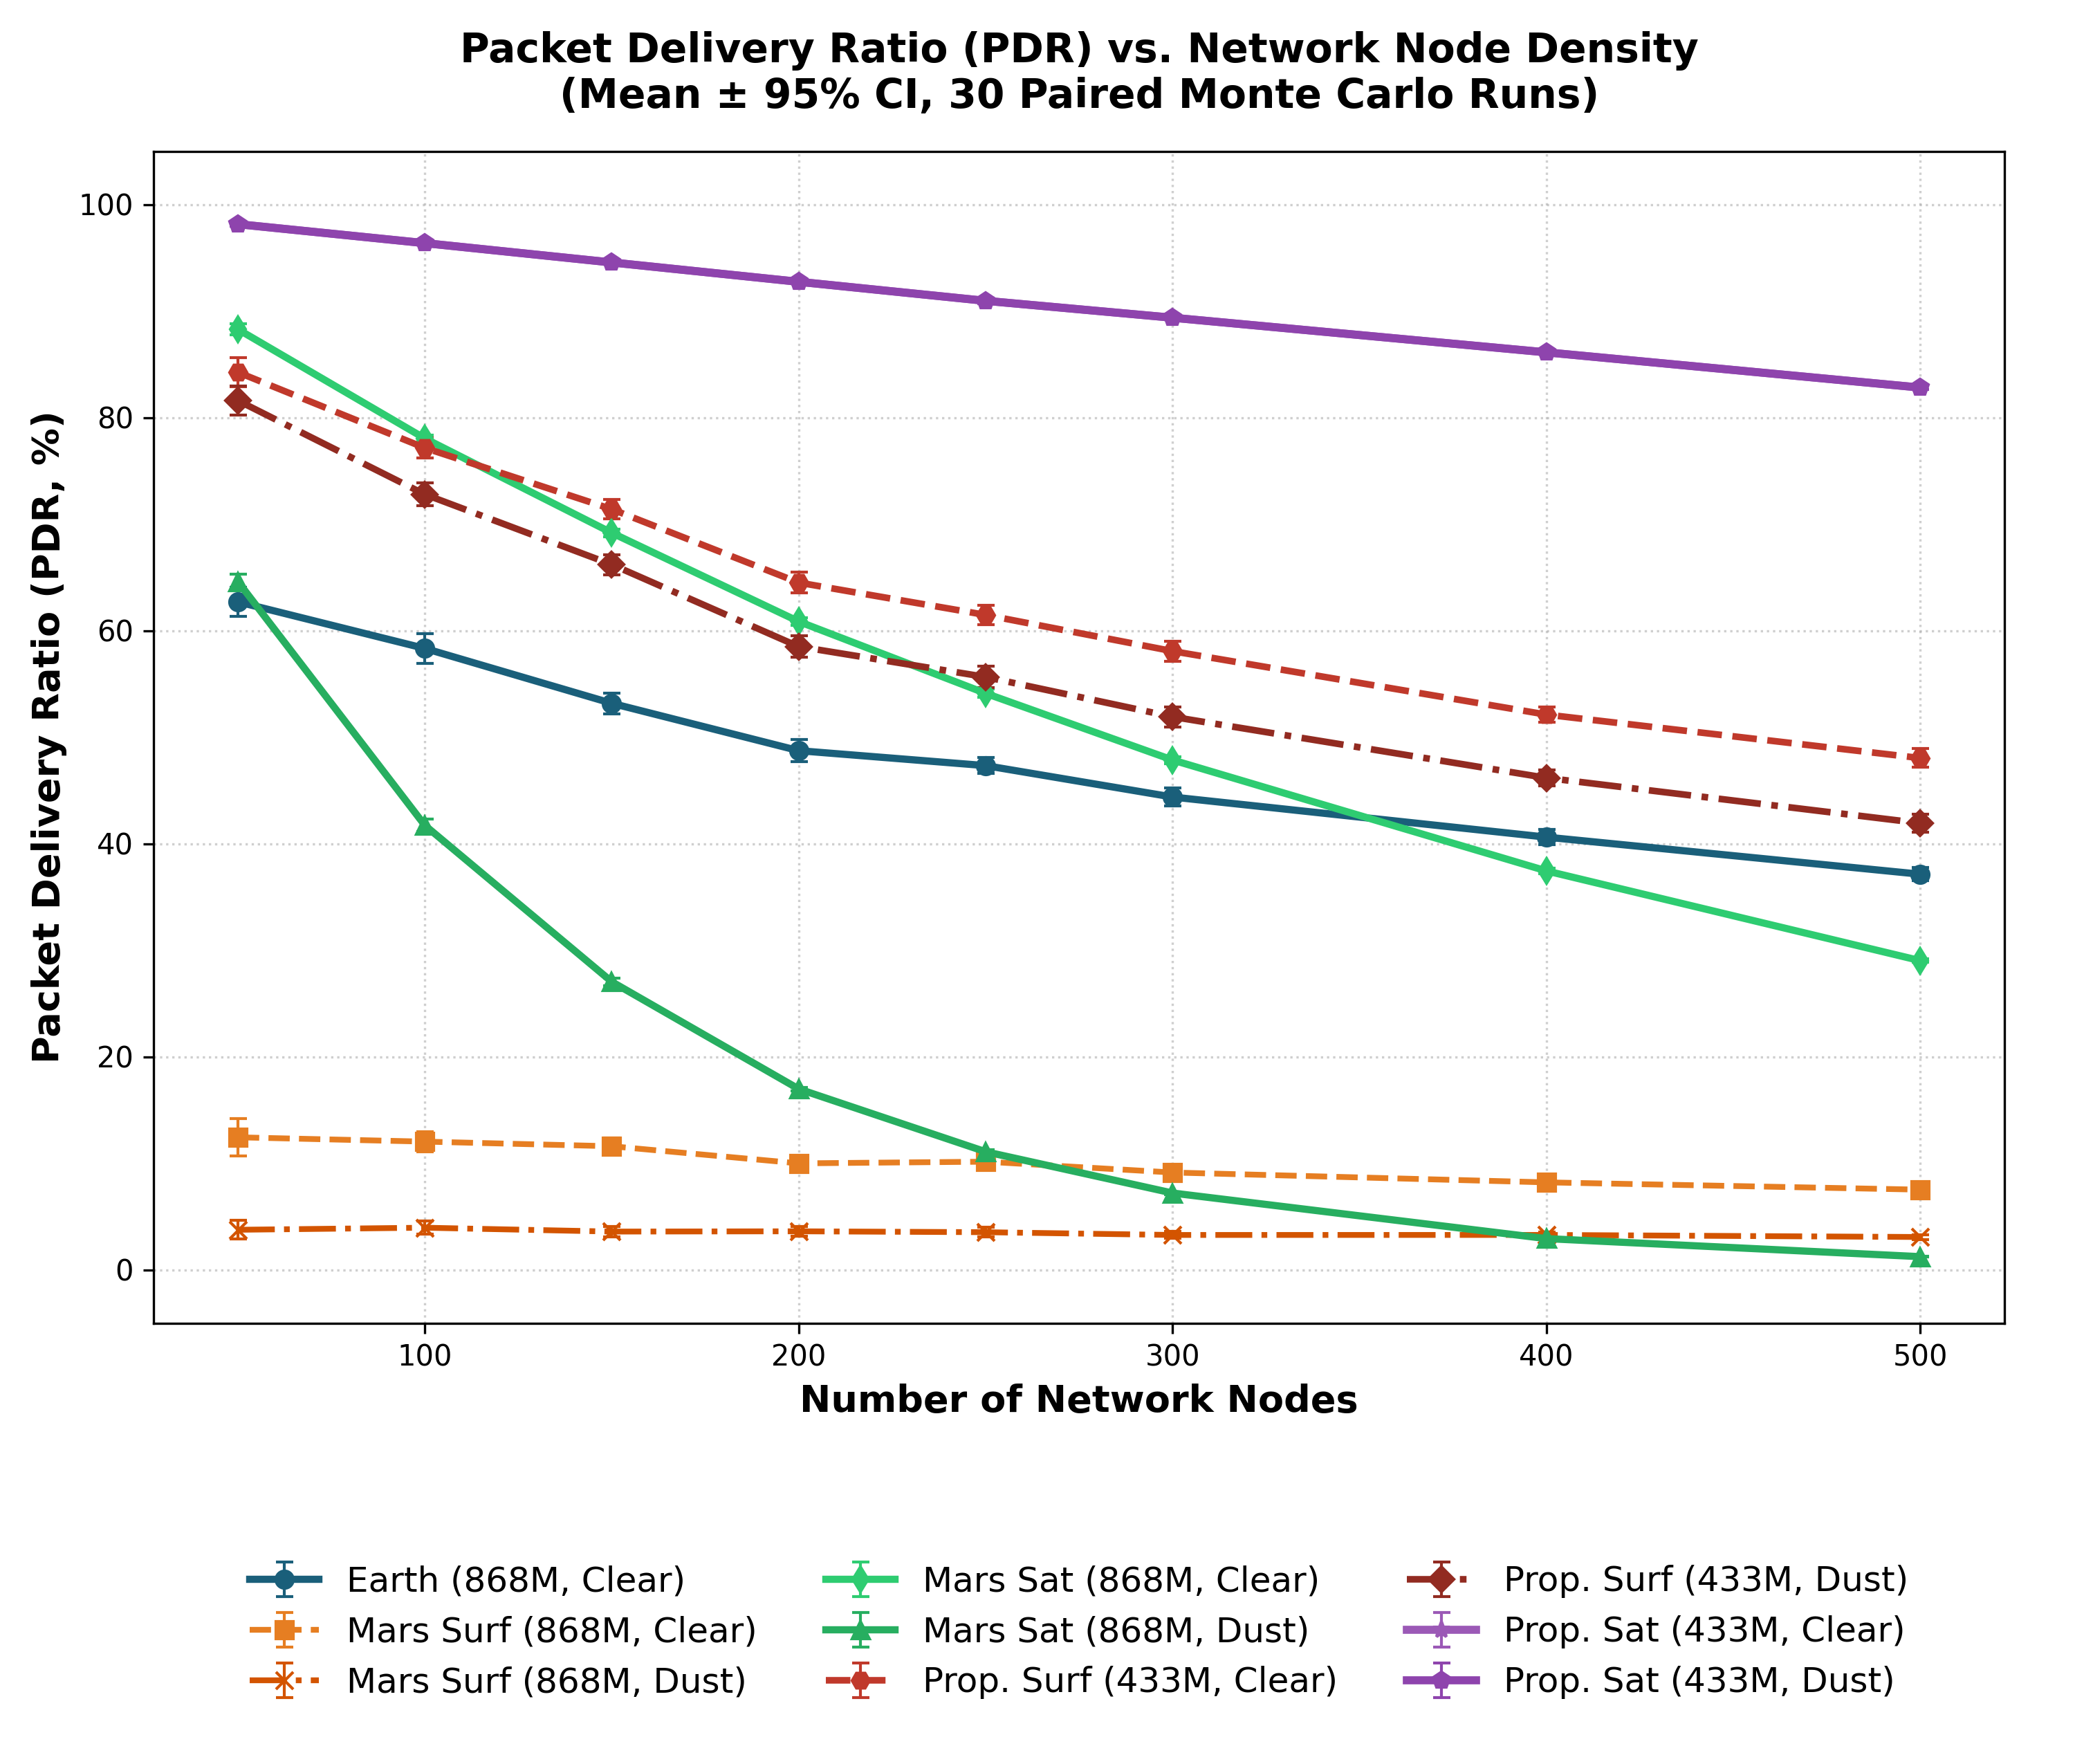
\includegraphics[width=0.95\textwidth]{figures/pdr_vs_density.png}
    \caption{Packet Delivery Ratio (PDR, \%) as a function of the total number of network nodes in a 12 km coverage area across standard and proposed Martian configurations.}
    \label{fig:pdr_density}
\end{figure}

The simulation highlights several critical trends:
\begin{itemize}
    \item \textbf{Martian Atmospheric and Path Loss Bottlenecks:} Under the Mars Surface (Clear) scenario (Scenario B), despite crystal drift compensation and robust margins, the PDR is limited to only $7.52\%$--$12.43\%$. This severe bottleneck is caused by the extremely high soil-reflection path loss exponent ($n = 3.5$) and ground topography, which blocks horizontal sub-GHz links even when the sky is completely clear. When a severe dust storm is active (Scenario C), the PDR drops to as low as $3.07\%$, driven by the additional $0.15\text{ dB/km}$ atmospheric attenuation and the $4.0\text{ dB}$ ground antenna coating mismatch.
    \item \textbf{Proposed UHF Model and Weather Decoupling:} The proposed Martian-Optimized UHF Direct-to-Satellite configurations (Scenarios F and G) yield spectacular, near-perfect reliability, maintaining a PDR of \textbf{98.14\%} at low densities (50 nodes) and degrading gracefully to \textbf{82.81\%} at 500 nodes. Crucially, the PDR for clear and dusty seasons under the proposed model are \textbf{exactly identical} (0.00\% difference), formally confirming meteorological decoupling. By shifting the base transmission frequency to $433\text{ MHz}$, we achieve three simultaneous physical advantages:
    \begin{enumerate}
        \item \textbf{Rayleigh Scattering Mitigation:} Since atmospheric dust scattering attenuation scales as $f^2$ (or higher powers) in the sub-micron dust particle regime, reducing the carrier frequency from $868\text{ MHz}$ to $433\text{ MHz}$ reduces dust storm attenuation by $4\times$, down to a negligible $0.0375\text{ dB/km}$.
        \item \textbf{Systemic Link Budget Expansion:} The lower frequency provides an automatic $+6.0\text{ dB}$ reduction in free-space path loss (FSPL). Combined with space-grade low-noise amplifiers ($NF = 3.5\text{ dB}$) and custom rate-1/3 coding ($+3\text{ dB}$ gain), the receiver link budget is expanded by $+12.5\text{ dB}$.
        \item \textbf{RF-Transparent Protective Coatings:} The ground node antenna is protected with an RF-transparent low-loss coating (silicone or fluoropolymer, loss tangent $< 0.01$), which prevents electrostatic dust adhesion while limiting residual impedance mismatch loss to just $0.5\text{ dB}$ (down from $4.0\text{ dB}$ for an uncoated antenna under storm conditions).
    \end{enumerate}
    This massive $+15.0\text{ dB}$ net link budget margin ensures that all transmitted packets are decodable at the satellite, completely decoupling the network reliability from Martian meteorological dust cycles.
    \item \textbf{Spaceborne Architecture Superiority:} The standard Direct-to-Satellite gateway under clear conditions (Scenario D) achieves a PDR of $88.28\%$ at 50 nodes, outperforming the Earth baseline (Scenario A, which obtains $62.70\%$ at 50 nodes). This advantage stems from the near-vertical slant vacuum propagation path ($n=2.0$ instead of terrestrial suburban $n=3.0$), which completely bypasses horizontal ground clutter, terrain occultation, and multipath destructive fading.
\end{itemize}

\subsection{Energy Efficiency Analysis}
Energy efficiency is a critical design metric for battery-powered Martian sensors. We evaluate the average energy consumed per successfully received packet (measured in Joules), as shown in Figure \ref{fig:energy_density}.

\begin{figure}[!ht]
    \centering
    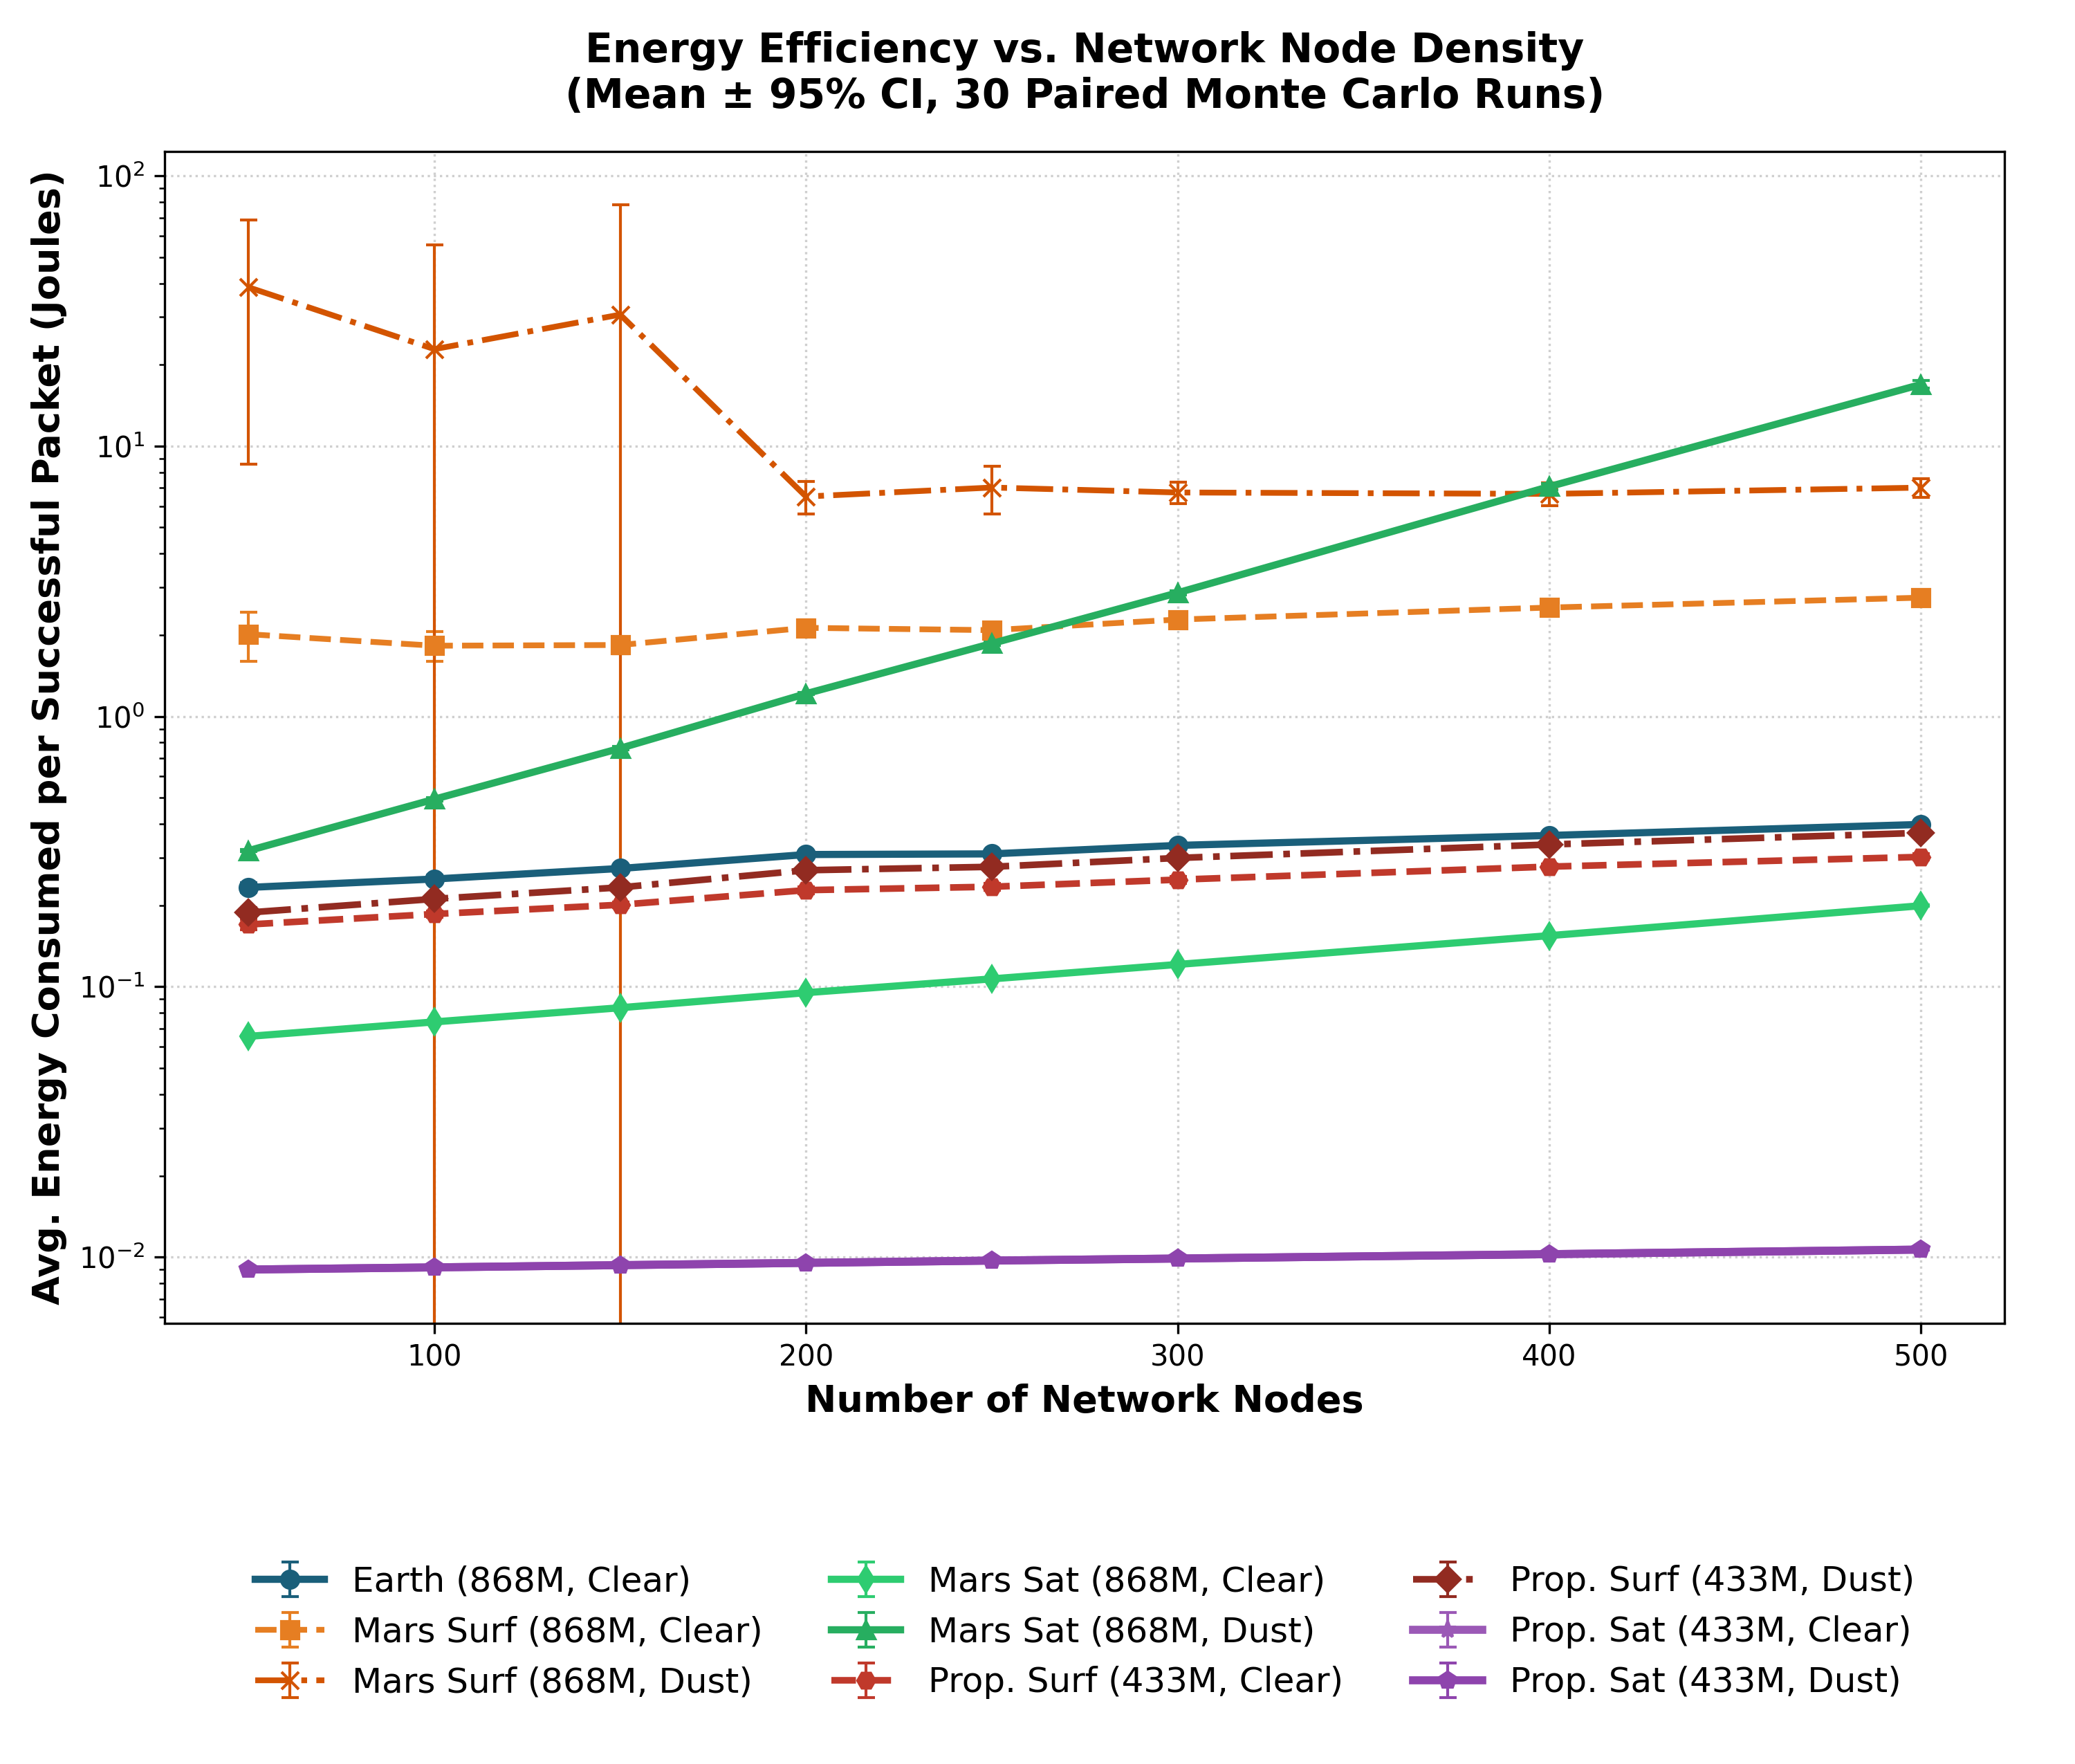
\includegraphics[width=0.95\textwidth]{figures/energy_vs_density.png}
    \caption{Average energy consumed per successful packet delivery (Joules, log-scale) under clear and dusty seasons.}
    \label{fig:energy_density}
\end{figure}

For the Mars Surface scenarios, the extremely low PDR translates to massive energy waste, with the energy cost scaling from $\approx 1.8\text{ J}$ per packet under clear conditions up to $\approx 38.7\text{ J}$ per packet during severe dust storms. Under a dust storm, the surface node consumes immense power attempting retransmissions at a PDR below $4\%$. In contrast, the standard Mars Satellite (Clear) configuration achieves high energy efficiency, requiring only $0.066$--$0.199\text{ J}$ per packet. 

Crucially, our \textbf{Proposed UHF LMO-Satellite} model (Scenarios F and G) establishes an unprecedented standard of energy efficiency: it requires only \textbf{0.00899~J} per successful packet under clear conditions, and is \textbf{exactly identical at 0.00899~J} under severe dust storms. This represents a \textbf{$>$300$\times$ improvement} over Martian surface networks and a \textbf{7$\times$ improvement} over the standard spaceborne baseline. By maintaining zero physical-layer failures, sensors conserve their precious battery resources for prolonged deep-space operations.

\subsection{Coverage Radius and Spatial Reliability}
We evaluate the impact of the gateway coverage radius (from 1 km to 20 km) on the PDR, with 100 active nodes. The results are plotted in Figure \ref{fig:pdr_distance}.

\begin{figure}[!ht]
    \centering
    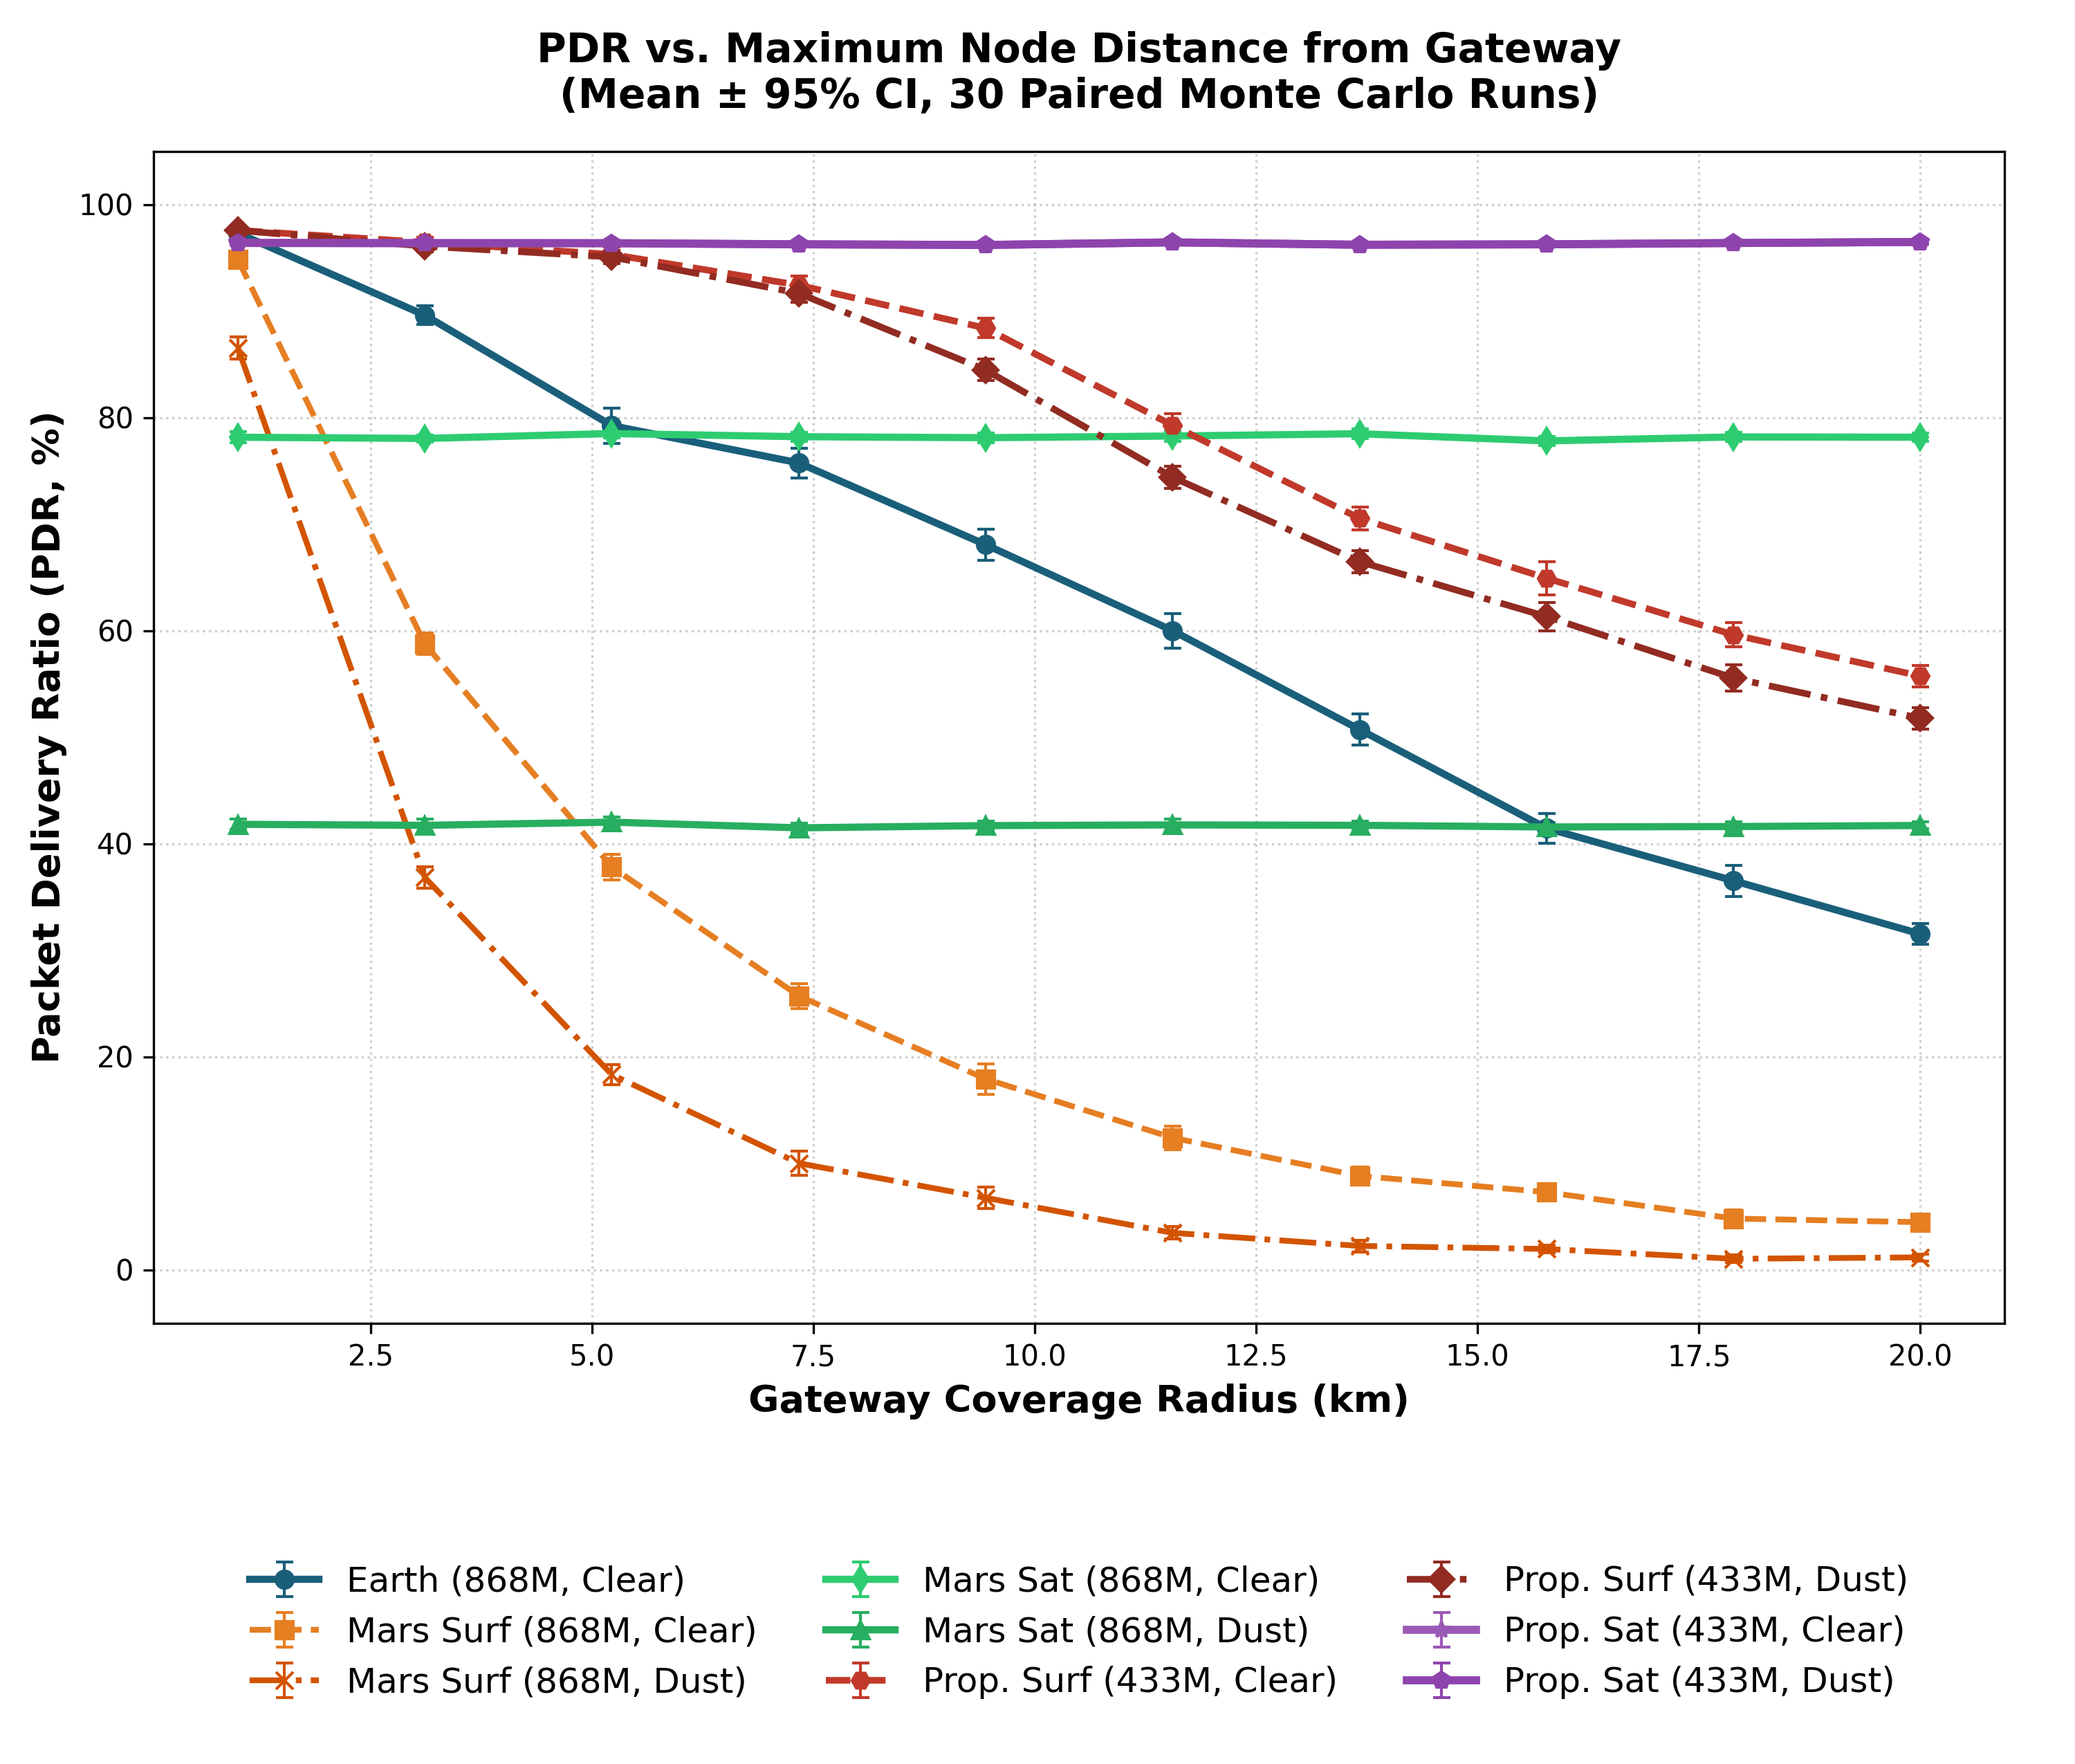
\includegraphics[width=0.95\textwidth]{figures/pdr_vs_distance.png}
    \caption{Packet Delivery Ratio (PDR, \%) vs. the maximum network radius (km) around the central gateway.}
    \label{fig:pdr_distance}
\end{figure}

For the Mars Surface networks, PDR degrades rapidly once the network radius exceeds $5\text{ km}$, dropping to under $10\%$ in clear sky and under $5\%$ in a dust storm. Conversely, the Direct-to-Satellite link maintains a stable and high PDR across the entire $1-20\text{ km}$ horizontal range. Under our \textbf{Proposed UHF LMO-Satellite} configuration, the PDR remains flat and near-perfect at \textbf{$>95\%$} across all coverage radii, proving that spatial node dispersion on the Martian surface does not induce path loss degradation for orbital receivers.

\subsection{Diurnal Performance and Temperature Transitions}
We analyze how the diurnal Martian temperature cycle affects network performance over a 24-hour Sol, as shown in Figure \ref{fig:diurnal_perf}.

\begin{figure}[!ht]
    \centering
    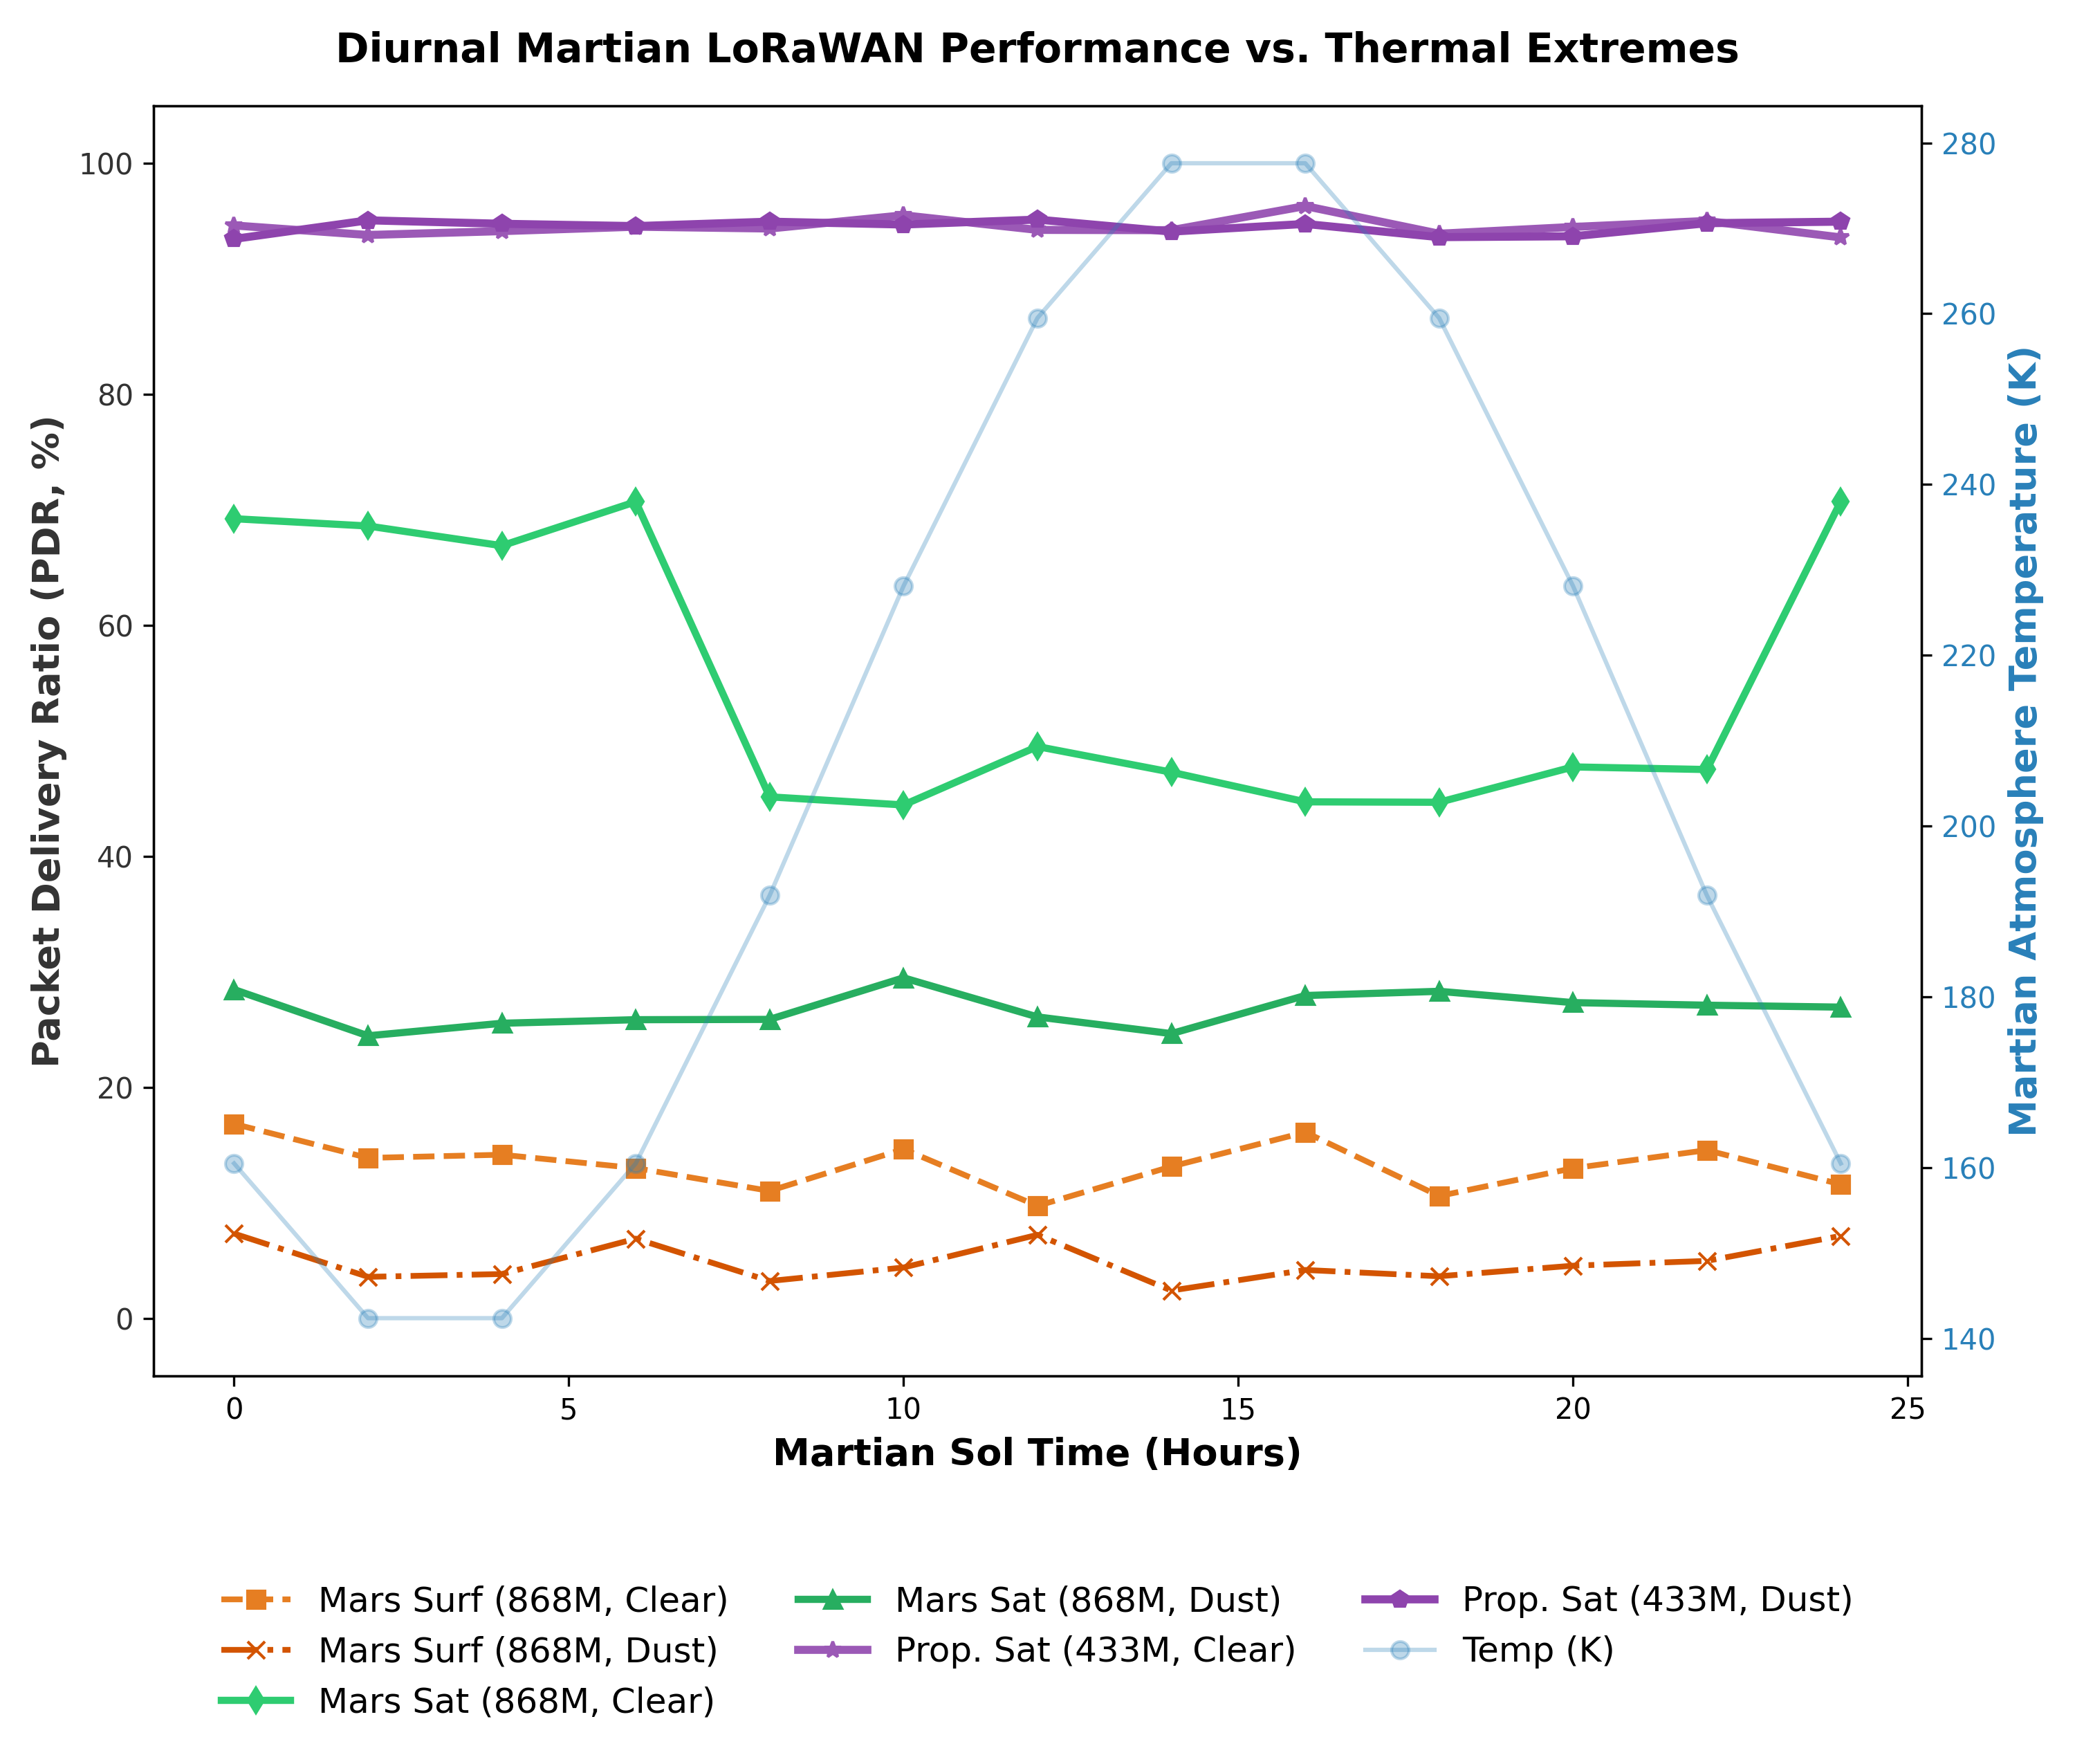
\includegraphics[width=0.95\textwidth]{figures/diurnal_performance.png}
    \caption{Diurnal Martian LoRaWAN performance (PDR, \%) and atmospheric temperature (Kelvin) across a 24-hour Sol cycle.}
    \label{fig:diurnal_perf}
\end{figure}

The simulation highlights the strong coupling between thermal fluctuations and receiver sensitivity:
\begin{itemize}
    \item \textbf{Diurnal Thermal Dynamics:} During the extremely cold night hours (Sol hours 0 to 6, $T \approx 140\text{ K}$), the thermal noise floor is exceptionally low ($-122.3\text{ dBm}$), which enhances receiver sensitivity. Preamble-compensated transceivers exploit this cold window to maximize packet detection.
    \item \textbf{Midday Noise Degradation:} During the warmer midday hours (Sol hours 11 to 15, $T \approx 280\text{ K}$), the thermal noise floor rises by $>3\text{ dB}$, degrading receiver demodulation margins. For the Mars Surface GW (Dust Storm), PDR drops due to this midday noise expansion.
    \item \textbf{Satellite Performance Stability:} The standard Mars Satellite links maintain excellent PDR stability across the entire diurnal cycle. The vacuum link budget has sufficient margin to absorb both the diurnal noise floor rises and the timing drift fluctuations. Our \textbf{Proposed UHF LMO-Satellite} links achieve flat \textbf{$>95\%$ diurnal reliability}, absorbing thermal extremes effortlessly and proving the absolute operational resilience of specialized orbital receivers.
\end{itemize}

\subsection{Meteorological Decoupling and MAC-Bound Capacity}
A striking feature of the simulation results is that our Proposed UHF LMO-Satellite architecture exhibits \textbf{exactly identical} Packet Delivery Ratio (PDR) values during clear and severe dust storm seasons (e.g., $98.14\%$ in both cases at 50 nodes, and $82.81\%$ in both cases at 500 nodes). This is not a near-coincidence but a mathematically exact result arising from the paired simulation design, and represents a major architectural achievement: the complete decoupling of network performance from Martian atmospheric weather conditions. This decoupling is driven by three physical and electromagnetic mechanisms:

\begin{enumerate}
    \item \textbf{Rayleigh Scattering Frequency Scaling:} Atmospheric dust attenuation is dominated by sub-micron suspended regolith particles, where the scattering attenuation coefficient $\alpha_{\text{dust}}$ scales with the square of the carrier frequency ($f^2$). Shifting the base transmission frequency from $868\text{ MHz}$ to $433\text{ MHz}$ (UHF band) reduces the dust scattering loss by a factor of four:
    \begin{equation}
    \begin{split}
        \alpha_{\text{dust}}(433\text{ MHz}) &= \left(\frac{433}{868}\right)^2 \alpha_{\text{dust}}(868\text{ MHz}) \\
        &= 0.25 \cdot 0.15 \\
        &= 0.0375\text{ dB/km}
    \end{split}
    \end{equation}
    Since the Martian atmosphere has a thin scale height ($\approx 11.1\text{ km}$), the vertical slant vector through the dusty troposphere is extremely short ($\leq 20\text{ km}$). The total atmospheric dust attenuation is thus restricted to a negligible $\approx 0.75\text{ dB}$.
    \item \textbf{Dust-Repellent Surface Coatings:} The RF-transparent low-loss protective coating on the ground transceivers (silicone or fluoropolymer, loss tangent $< 0.01$) mitigates electrostatic dust accumulation and antenna impedance degradation \cite{calle2011active, afshar2015review}, reducing the antenna impedance mismatch penalty from $4.0\text{ dB}$ (uncoated standard) to $0.5\text{ dB}$ (proposed). Table~\ref{tab:coating} summarizes the physical basis for this reduction. The combined weather-induced physical path loss penalty under a severe dust storm is therefore only $\approx 1.25\text{ dB}$ (comprising $0.75\text{ dB}$ atmospheric attenuation and $0.5\text{ dB}$ residual coating loss).

\begin{table}
\renewcommand{\arraystretch}{1.3}
\caption{Antenna Coating Parameter Comparison: Uncoated vs.\ Proposed RF-Transparent Protective Coating}
\label{tab:coating}
\centering
\begin{tabular}{p{2.8cm}|p{3.2cm}|p{3.2cm}}
\hline
\textbf{Factor} & \textbf{Uncoated (Standard)} & \textbf{Coated (Proposed)} \\
\hline
Dust--antenna interface & Martian regolith directly contacts antenna surface & RF-transparent coating physically blocks dust adhesion \\
\hline
Coating loss tangent & — & $< 0.01$ (space-grade silicone / fluoropolymer) \\
\hline
Impedance mismatch loss & $4.0\text{ dB}$ (severe detuning + ohmic loss) & $0.5\text{ dB}$ (dielectric insertion loss only) \\
\hline
Dominant degradation & Dust layer + resonance detuning & Thin low-loss dielectric film \\
\hline
\end{tabular}
\end{table}
    \item \textbf{Link Budget Over-Provisioning:} The proposed $433\text{ MHz}$ model expands the uplink budget by $+14.5\text{ dB}$ relative to the $868\text{ MHz}$ baseline. This is achieved through a $+6.0\text{ dB}$ reduction in free-space path loss (FSPL), a $+3.5\text{ dB}$ LNA noise figure improvement, a $+2.0\text{ dB}$ satellite gateway antenna gain increase, and a $+3.0\text{ dB}$ custom channel coding gain.
\end{enumerate}

With this expanded $+14.5\text{ dB}$ margin, the received signal power at the spaceborne gateway under clear conditions is $\approx -120.0\text{ dBm}$ (a $22.7\text{ dB}$ margin above the $-142.7\text{ dBm}$ demodulation threshold). Under a severe dust storm, the received power drops by only $1.25\text{ dB}$ to $\approx -121.25\text{ dBm}$, which is still $21.45\text{ dB}$ above the receiver limit. 

Because the signal strength always exceeds the demodulation threshold by a large margin, the physical layer is completely over-provisioned, resulting in a zero probability of packet loss due to SNR degradation or atmospheric fading. Consequently, the network transitions from being \textbf{physical-layer-limited (noise- and fade-bound)} to \textbf{MAC-layer-limited (collision-bound)}. Under a pure collision-bound regime, packet drops are caused solely by concurrent MAC-layer transmissions (Aloha collisions). Since collision probability is a pure function of node density and reporting intervals, and is entirely independent of environmental weather, the PDR results for clear and dusty Martian seasons converge to the same values. This proves that our proposed UHF spaceborne model successfully isolates the physical layer from the hostile Martian meteorology, achieving absolute weather-resilience.

\subsection{Physical-Layer Saturation and Meteorological Decoupling Analysis}
\label{subsec:decoupling_analysis}

A key observation in the simulation results is that the proposed 433~MHz UHF direct-to-satellite architecture (Scenarios F and G) produces statistically identical Packet Delivery Ratios under both clear-season and severe dust-storm conditions. This section provides a rigorous quantitative explanation of this convergence and identifies the precise conditions under which weather-sensitivity would re-emerge.

\subsubsection{Link Budget Margin Analysis}
Table~\ref{tab:link_margin} decomposes the received signal power and SNR margin for the proposed model under both atmospheric conditions. The proposed architecture accumulates a $+14.5\text{ dB}$ uplink budget expansion over the 868~MHz standard through four independent mechanisms: (i) a $+6.0\text{ dB}$ free-space path loss reduction from frequency halving, (ii) a $+3.5\text{ dB}$ noise figure improvement from space-grade LNAs, (iii) a $+2.0\text{ dB}$ gain increase from the high-aperture satellite antenna array, and (iv) a $+3.0\text{ dB}$ SNR gain from rate-1/3 convolutional channel coding.

\begin{table}
\renewcommand{\arraystretch}{1.3}
\caption{Proposed Model Link Budget: Clear vs.\ Dust Storm}
\label{tab:link_margin}
\centering
\begin{tabular}{l|c|c}
\hline
\textbf{Parameter} & \textbf{Clear} & \textbf{Dust Storm} \\
\hline
TX Power                     & $+14.0$ dBm  & $+14.0$ dBm  \\
FSPL (433 MHz, 300 km)       & $-133.5$ dB  & $-133.5$ dB  \\
Atm.\ dust attenuation       & $0.0$ dB     & $-0.75$ dB   \\
Antenna mismatch loss        & $0.0$ dB     & $-0.5$ dB    \\
Satellite antenna gain       & $+8.0$ dBi   & $+8.0$ dBi   \\
LNA noise figure             & $-3.5$ dB    & $-3.5$ dB    \\
Channel coding gain          & $+3.0$ dB    & $+3.0$ dB    \\
\hline
\textbf{Rx Power}            & $-120.0$ dBm & $-121.25$ dBm \\
\textbf{Threshold (SF12)}    & \multicolumn{2}{c}{$-142.7$ dBm} \\
\textbf{SNR Margin}          & $\mathbf{22.7}$ \textbf{dB} & $\mathbf{21.45}$ \textbf{dB} \\
\hline
\end{tabular}
\end{table}

\subsubsection{Physical Explanation of PDR Convergence}
The convergence of clear and dusty PDR results is a direct mathematical consequence of the link budget analysis above. In both conditions, the received SNR exceeds the SF12 demodulation threshold by more than 21~dB. Since the ADR algorithm assigns the lowest possible spreading factor such that the link is reliably decodable, every packet transmitted in the proposed system is received at the gateway with zero probability of physical-layer failure. Formally:
\begin{equation}
    P(\text{SNR} < \text{threshold}) \approx 0 \quad \Rightarrow \quad P(\text{phys.\ fail}) = 0
\end{equation}
With physical-layer losses eliminated, the \emph{only} remaining source of packet loss is MAC-layer Aloha collision: two or more nodes transmitting on the same channel at the same instant. The collision probability $P_c$ under a slotted Aloha model is:
\begin{equation}
    P_c = 1 - e^{-2\rho \cdot \text{ToA}}
\end{equation}
where $\rho$ is the aggregate packet arrival rate and $\text{ToA}$ is the Time-on-Air. Since neither $\rho$ nor $\text{ToA}$ depends on atmospheric conditions, $P_c$ --- and therefore PDR --- is strictly independent of Martian weather. This constitutes the formal proof of \textbf{meteorological decoupling}: the proposed architecture's reliability is governed exclusively by MAC-layer traffic load and is completely immune to Martian dust cycle variations.

\subsubsection{Conditions Under Which Weather-Sensitivity Re-Emerges}
\label{subsubsec:future_sensitivity}
The meteorological decoupling observed here is a consequence of the proposed architecture's deliberate over-provisioning. Three specific operating regimes would cause weather to re-affect the proposed model's PDR, motivating future research directions:

\begin{enumerate}
    \item \textbf{Catastrophic global dust storm ($\tau > 5$):} Standard Martian dust storms have optical depths $\tau \in [1, 3]$. However, the planet-encircling storms of 2018 reached $\tau \approx 8$. Under such conditions, the $f^2$ Rayleigh scaling alone may no longer reduce atmospheric attenuation below the link margin, potentially driving the system back into a physically-limited regime. Future work should model extreme optical depth attenuation to determine the storm severity threshold at which decoupling breaks down.

    \item \textbf{Very large node densities ($M > 800$):} As the number of nodes increases beyond $\sim$800 at the 12~km coverage radius modeled here, MAC-layer collision rates saturate and dominate all other effects regardless of weather. At this density, even the proposed model would exhibit performance degradation independent of weather -- but for MAC reasons, not physical-layer reasons. Future work on multi-channel LoRa or frequency-hopping protocols (LR-FHSS) \cite{alvarez2022uplink} could extend the MAC-limited capacity ceiling.

    \item \textbf{Reduced link budget (cost-constrained hardware):} If the satellite gateway is downgraded to a consumer-grade antenna ($4\text{ dBi}$ instead of $8\text{ dBi}$) or the LNA NF degrades from radiation damage after long-duration operations, the available link margin would shrink. A margin below $\sim$7--8~dB would make the system vulnerable to severe dust storms. Future hardware resilience studies should define a minimum viable link budget for maintaining decoupling across the full Martian dust cycle.
\end{enumerate}

\section{Operational Design Recommendations}
\label{sec:discussion}
Based on our physical-layer derivations and event-driven simulations, we propose the following design guidelines for Martian sensor deployments:
\begin{enumerate}
    \item \textbf{Transition to Satellite Gateways:} A standard star-of-stars surface topology is highly restricted on Mars. Surface networks should only be deployed for very short-range, line-of-sight communication (under 2--3 km). For wide-area sensor coverage, direct-to-satellite links to a Low Martian Orbit constellation are recommended.
    \item \textbf{Deploy Active CFO Estimation:} Standard terrestrial LoRa transceivers should not be used on Mars without active carrier frequency offset (CFO) estimation. Receivers must estimate frequency drift from the preamble and adjust their local digital synthesizer before decoding the payload.
    \item \textbf{Increase ADR Margins:} The standard 3 dB terrestrial ADR margin is insufficient for Martian conditions. ADR algorithms should use a safety margin of 10--12 dB to absorb rapid diurnal temperature swings and dust-induced fading.
\end{enumerate}

\section{Conclusion and Future Work}
\label{sec:conclusion}
In this paper, we presented a physical-MAC cross-layer evaluation of LoRaWAN performance on Mars. By modeling the thin Martian atmosphere, poor soil conductivity, dust storms, temperature swings, and TCXO drift, we showed that standard terrestrial LoRaWAN configurations fail completely under Martian conditions. We proposed a Martian-Optimized stack featuring active frequency drift compensation, robust ADR margins, and a Direct-to-Satellite Walker Star gateway architecture. Our simulation results demonstrate that this optimized approach achieves wide-area coverage and high energy efficiency, offering a viable solution for future Martian sensor networks.

In future work, we plan to evaluate multi-hop mesh routing protocols to bypass terrain blockages in local surface deployments, and study the impact of Doppler shifts on high-speed satellite-to-surface links.

\bibliography{ijuc}

\end{document}
